\documentclass[11pt,a4paper]{article}

% --------------------------------------------------
% Packages
% --------------------------------------------------
\usepackage[margin=2cm]{geometry}
\usepackage[utf8]{inputenc}
\usepackage[T1]{fontenc}
\usepackage{amsmath}
\usepackage{tabularx}
\usepackage{longtable}
\usepackage{caption}
\captionsetup{font=small,labelfont=bf}
\setlength{\emergencystretch}{2em}
\usepackage{graphicx}
\graphicspath{{figures/}}
\usepackage{pdflscape}
\usepackage{xcolor}
\usepackage{array}
\newcolumntype{P}[1]{>{\raggedright\arraybackslash}p{#1}}
\newcolumntype{Y}{>{\raggedright\arraybackslash}X}
\usepackage{booktabs}
\usepackage{float}
\usepackage{hyperref}
\usepackage{setspace}
\usepackage{tikz}
\usepackage{indentfirst}
\usepackage{tcolorbox}
\tcbuselibrary{breakable}
\usepackage[round]{natbib}

% --------------------------------------------------
% Paragraph formatting
% --------------------------------------------------
\setlength{\parindent}{1.25cm}
\setlength{\parskip}{0pt}

% --------------------------------------------------
% Colors
% --------------------------------------------------
\definecolor{mainblue}{HTML}{1c3c88}
\definecolor{lightblue}{HTML}{00682E}
\definecolor{darkgray}{HTML}{333333}
\definecolor{softgray}{HTML}{F5F5F5}
\definecolor{infobackground}{HTML}{EAF2F8}
\renewcommand{\contentsname}{\textcolor{mainblue}{Contents}}

% --------------------------------------------------
% Document metadata
% --------------------------------------------------
\newcommand{\manualreviewdate}{6 October 2026}
\newcommand{\testedqgisversion}{3.44.8}
\newcommand{\minimumqgisversion}{3.14}

% --------------------------------------------------
% Custom boxes
% --------------------------------------------------
\newtcolorbox{infobox}{
    colback=infobackground,
    colframe=mainblue,
    title=Information,
    fonttitle=\bfseries,
    arc=2mm,
    boxrule=0.8pt
}

\newcounter{tutorialstep}
\newcommand{\tutorialstep}[2]{%
    \refstepcounter{tutorialstep}%
    \par\medskip
    \noindent{\large\bfseries\color{mainblue}Step \thetutorialstep: #1}\par
    \vspace{0.15cm}
    \noindent #2\par
    \medskip
}

\newcommand{\screenshotplaceholder}[2]{%
    \begin{figure}[H]
        \centering
        \fcolorbox{lightblue}{softgray}{%
            \begin{minipage}[c][5.2cm][c]{0.88\textwidth}
                \centering
                {\Large\bfseries Screenshot to add}\\[0.35cm]
                #2
            \end{minipage}%
        }
        \caption{#2}
        \label{fig:#1}
    \end{figure}
}


% --------------------------------------------------
% Hyperlink setup
% --------------------------------------------------
\hypersetup{
    pdftitle={Best Fit Interpolator User Manual},
    pdfauthor={Best Fit Interpolator authors},
    colorlinks=true,
    linkcolor=black,
    urlcolor=mainblue,
    citecolor=mainblue
}

% --------------------------------------------------
% Document
% --------------------------------------------------
\begin{document}

% --------------------------------------------------
% Cover Page
% --------------------------------------------------
\begin{titlepage}

% Background soft frame
\begin{tikzpicture}[remember picture, overlay]
    \draw[line width=1.2pt, color=mainblue]
        ([xshift=1.2cm,yshift=-1.2cm]current page.north west)
        rectangle
        ([xshift=-1.2cm,yshift=1.2cm]current page.south east);

    \draw[line width=0.4pt, color=lightblue]
        ([xshift=1.45cm,yshift=-1.45cm]current page.north west)
        rectangle
        ([xshift=-1.45cm,yshift=1.45cm]current page.south east);
\end{tikzpicture}

\centering

\vspace*{1.2cm}

% Plugin logo
% Replace the file name with the actual plugin logo file in the figures folder

\includegraphics[width=0.28\textwidth]{plugin_logo.png}

\vspace{1cm}

% Main title
{\Huge \textbf{\color{mainblue}Best Fit Interpolator Plugin}}\\[0.4cm]

{\Large \textbf{User Tutorial and Practical Guide}}\\[0.45cm]

% Short description
\begin{minipage}{0.82\textwidth}
\centering
\onehalfspacing
{\large
A QGIS plugin for spatial mapping, interpolation method comparison, validation, and framework-based method recommendation.
}
\end{minipage}

\vspace{1.5cm}

% Technical information table
\renewcommand{\arraystretch}{1.35}
\begin{tabular}{>{\bfseries}P{5.2cm} P{7.2cm}}
\toprule
Document: & User manual \\
Last reviewed: & \manualreviewdate{} \\
QGIS compatibility: & QGIS \minimumqgisversion{} onward, including QGIS 4 \\
Software type: & QGIS Plugin \\
Language: & English \\
Scientific basis: & Framework article for interpolation method selection \\
\bottomrule
\end{tabular}

\vfill

% Author and institution
{\large \textbf{Laura Delgado Bejarano}}\\[0.15cm]
{\large \textbf{M.Sc. Agricultural Engineering -- Digital Agriculture}}\\[0.15cm]
{\large School of Agricultural Engineering -- University of Campinas}\\[0.15cm]
{\large Campinas, Brazil}\\[0.7cm]

% Logos at the bottom
\begin{minipage}{0.35\textwidth}
    \centering
    
\includegraphics[width=0.25\textwidth]{Gitap.png}\\[0.15cm]
    {\small \textit{Research group}}
\end{minipage}
\hfill
\begin{minipage}{0.35\textwidth}
    \centering
    
\includegraphics[width=0.42\textwidth]{qgis_logo.png}\\[0.15cm]
    {\small \textit{Developed for use in QGIS}}
\end{minipage}

\vspace{0.6cm}

{\large 2026}

\end{titlepage}

\begingroup
\hypersetup{linkcolor=black}
\tableofcontents
\endgroup
\newpage

% --------------------------------------------------
% Quick-start workflow overview
% --------------------------------------------------
\begin{landscape}
\phantomsection
\addcontentsline{toc}{section}{Quick Start Workflow}
\begin{figure}[H]
    \centering
    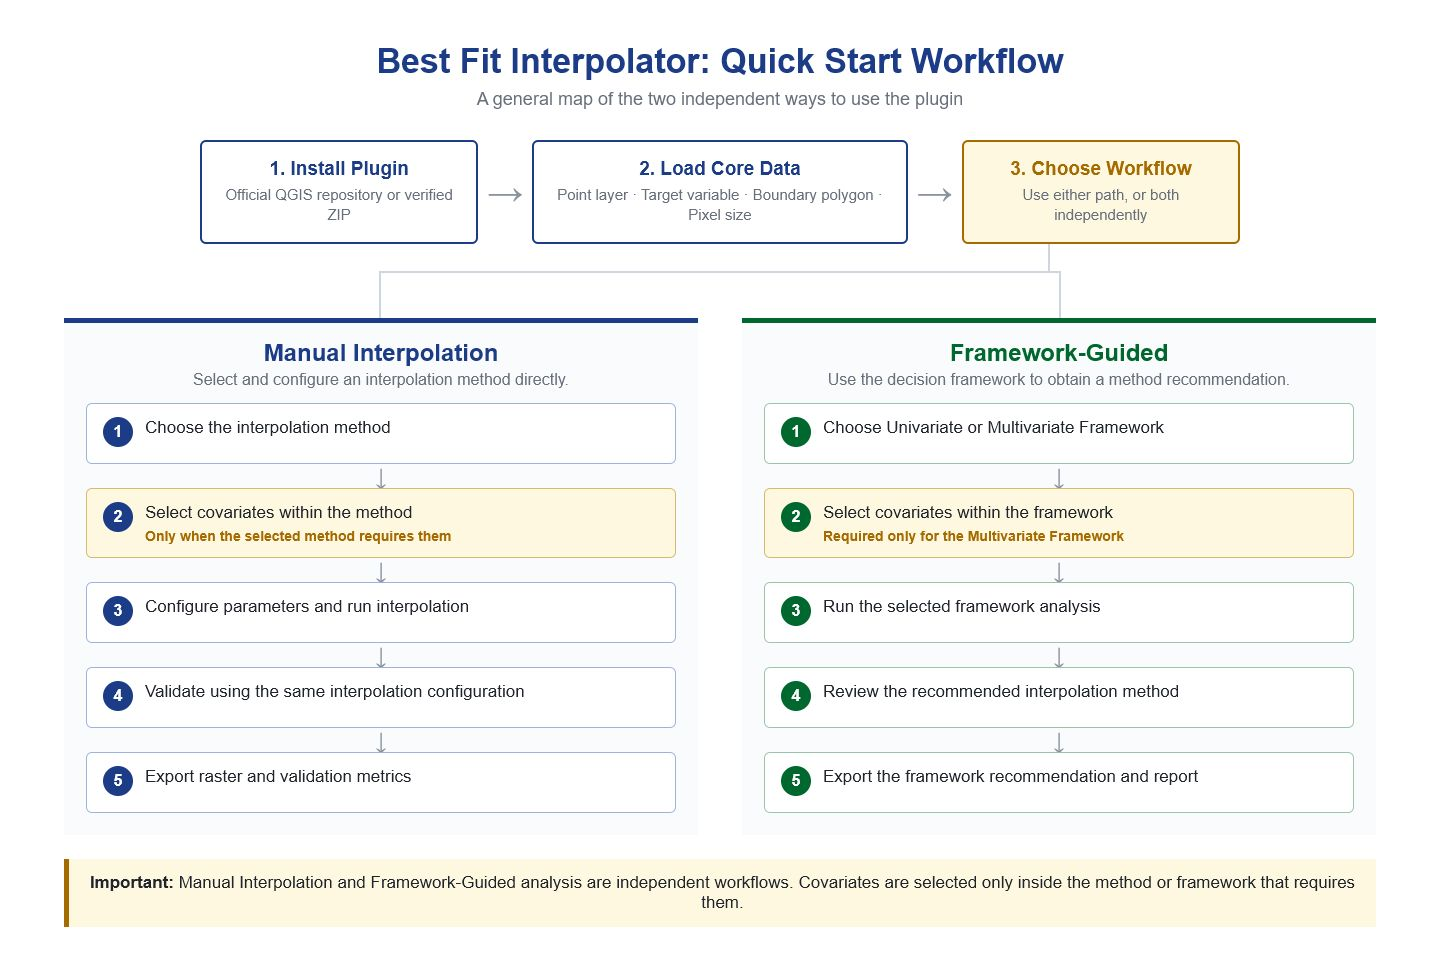
\includegraphics[width=0.98\linewidth,height=0.78\textheight,keepaspectratio]{quick_start_workflow.png}
    \caption{General workflow of the Best Fit Interpolator plugin. Manual Interpolation and Framework-Guided analysis are independent paths.}
    \label{fig:quick-start-workflow}
\end{figure}
\end{landscape}
\clearpage

% --------------------------------------------------
% Tutorial content
% --------------------------------------------------


\section{Motivation}

Spatial mapping is a fundamental step in many environmental, agricultural, and geospatial applications. Maps are used to represent the spatial distribution of variables, support decision-making, identify management zones, guide field operations, and communicate patterns that cannot be easily interpreted from point-based observations alone. However, producing a reliable map from sampled data is not a purely automatic task. The quality of the final map depends on several factors, including the number of samples, the spatial distribution of the sampling points, the spatial structure of the target variable, the interpolation method, and the validation strategy used to evaluate prediction performance.

In many practical situations, interpolation methods are selected based on habit, software availability, or visual appearance of the output map. This can lead to inconsistent results, especially when the characteristics of the dataset are not considered. A method that performs well for one variable, sampling density, or spatial pattern may not be suitable for another.

The \textit{Best Fit Interpolator Plugin} was developed to support a more transparent, reproducible, and data-driven interpolation workflow in QGIS. The plugin allows users to organize spatial input data, evaluate spatial diagnostics, apply different interpolation methods, compare validation metrics, and select a suitable method according to the characteristics of the dataset. Although the research framework behind the plugin was developed with soil data, the general problem addressed by the plugin is broader: how to choose an appropriate interpolation method for spatial mapping based on sample size, spatial pattern, spatial dependence, and prediction performance. Soil data were used as a case study because soil sampling is often limited by cost, making sampling density a critical factor in the mapping process.

This tutorial provides a step-by-step guide for using the plugin, from data preparation to final map export and report generation.

\section{What the Plugin Does}

The \textit{Best Fit Interpolator Plugin} integrates tools for spatial interpolation, validation, and method recommendation within QGIS. It was designed to help users perform a complete mapping workflow using point-based observations, boundary polygons, and, when available, auxiliary raster covariates.

The plugin can be applied to spatial mapping problems where the objective is to estimate a continuous surface from sampled observations. Although the framework was developed using soil attributes as the main case study, the plugin structure can support broader interpolation workflows involving different types of spatial variables.

\vspace{1cm}
The main functionalities include:

\begin{itemize}
    \item Selection of point-based observations, target variable, and boundary polygon;
    \item Definition of output pixel size;
    \item Global Moran's I, Local Moran / LISA, statistical outlier diagnostics, and explicit sample review;
    \item Deterministic interpolation methods, such as IDW and Thin Plate Spline;
    \item Geostatistical interpolation methods, including kriging-based approaches;
    \item Machine learning interpolation using auxiliary covariates;
    \item Validation and comparison of interpolation methods;
    \item Framework-based recommendation according to sample size, spatial pattern, and spatial dependence;
    \item Side-by-side maps and a signed difference map on a shared grid;
    \item Interactive session reports, temporary HTML previews, and PDF export;
    \item Automatic processing profiles for dense and massive datasets.
\end{itemize}

\section{Scientific Background}

The framework implemented in the \textit{Best Fit Interpolator Plugin} was developed based on the study by \citet{delgadobejarano2026}, published in \textit{Precision Agriculture}. The study evaluated how data characteristics, including sample size, sampling density, spatial structure, and spatial dependence, influence the performance and selection of interpolation methods for digital soil mapping. The scientific development of the framework was focused on soil mapping because soil sampling campaigns are often constrained by operational and economic costs. As a result, soil datasets commonly present different sampling densities, which directly affect interpolation performance and the uncertainty associated with the final map.

Despite this soil-based research context, the conceptual basis of the plugin is not restricted to soil fertility mapping. The central objective is to support users in understanding how the characteristics of their spatial data influence interpolation performance and method suitability.

The framework module uses spatial indicators, such as Moran's I, spatial pattern classification, and the spatial dependence index, together with validation metrics, to guide the recommendation of suitable interpolation methods. The original study proposed two decision frameworks: a univariate framework (Figure~\ref{fig:univariate_framework}), based mainly on the target variable and its spatial structure, and a multivariate framework (Figure~\ref{fig:multivariate_framework}), which also considers the use of auxiliary covariates.

\begin{infobox}
\textbf{Article citation}

The framework-based recommendation module implemented in the \textit{Best Fit Interpolator Plugin} is based on the following article:

\vspace{0.2cm}

DELGADO BEJARANO, L.; OLIVEIRA, A. L. G.; POZZUTO, J. V. F.; SÁNCHEZ, D. C.; AMARAL, L. R. do. Performance of interpolation methods in digital soil mapping: the influence of data characteristics. \textbf{Precision Agriculture}, v. 27, n. 1, article 10, 2026. DOI: \url{https://doi.org/10.1007/s11119-025-10311-8}.
\end{infobox}

\begin{figure}[H]
    \centering
    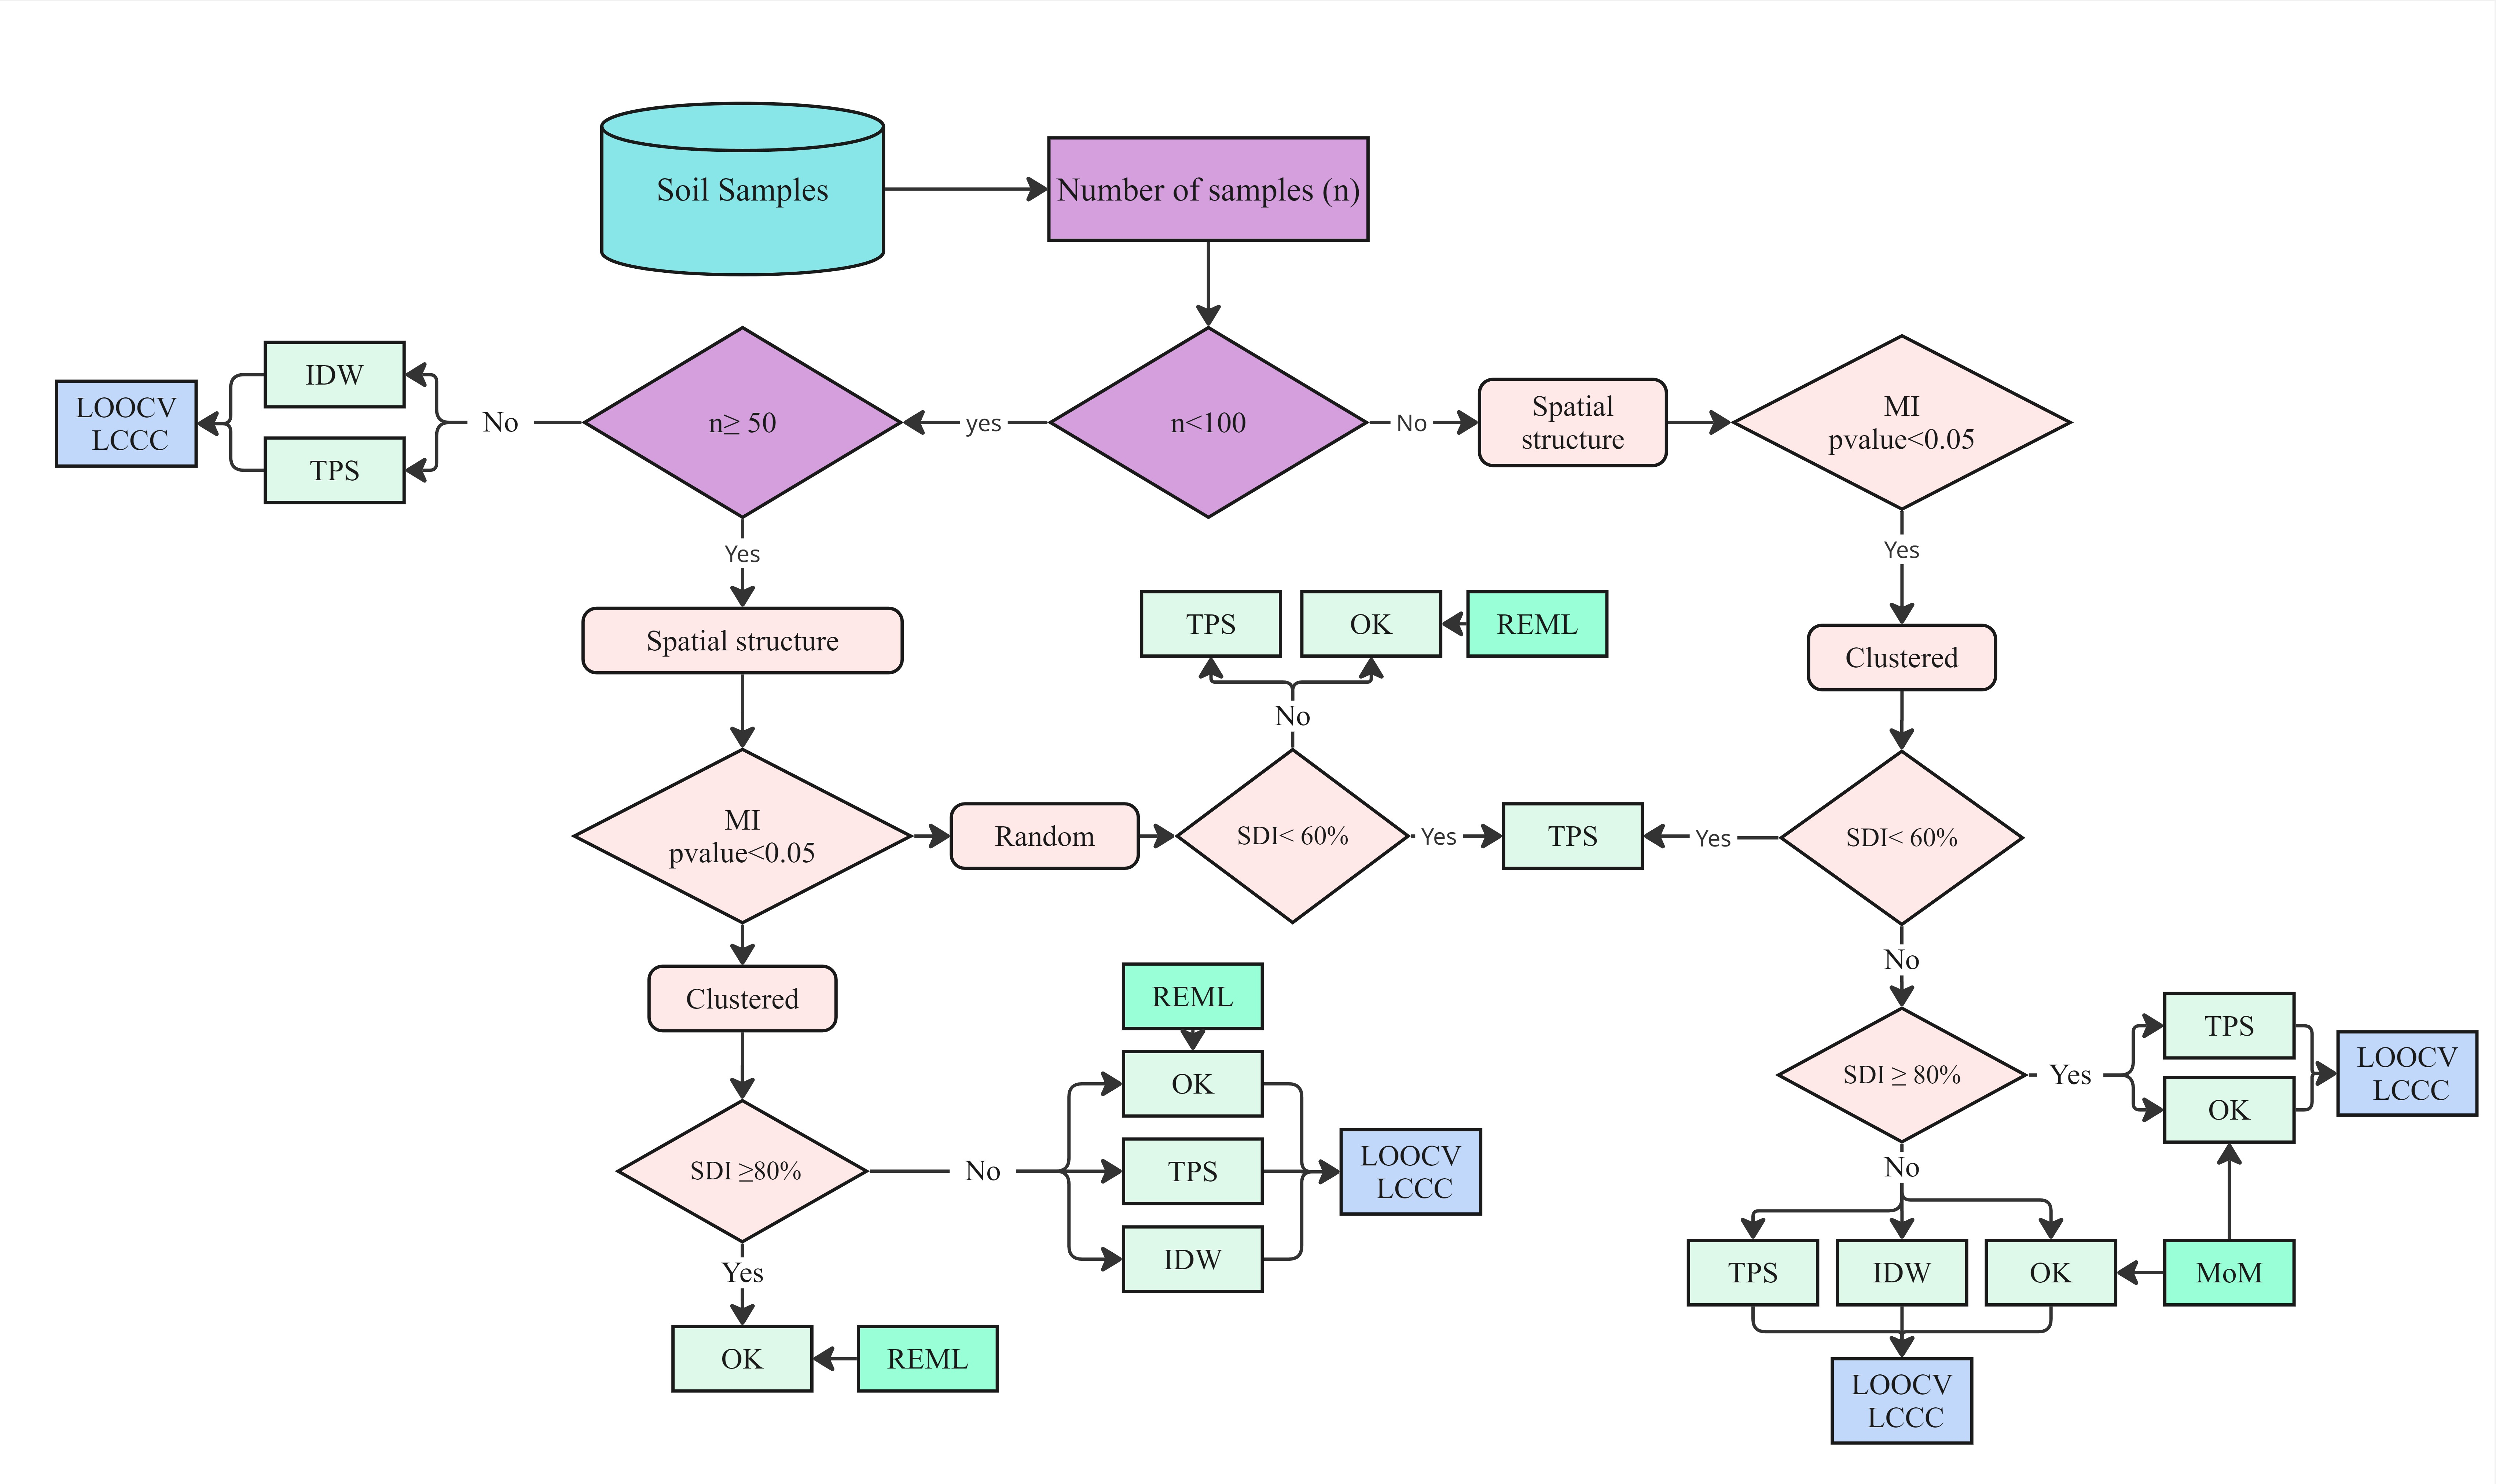
\includegraphics[width=0.95\textwidth]{univariate_framework.png}
    \caption{Univariate decision framework for interpolation method selection.}
    \label{fig:univariate_framework}
\end{figure}

\begin{figure}[H]
    \centering
    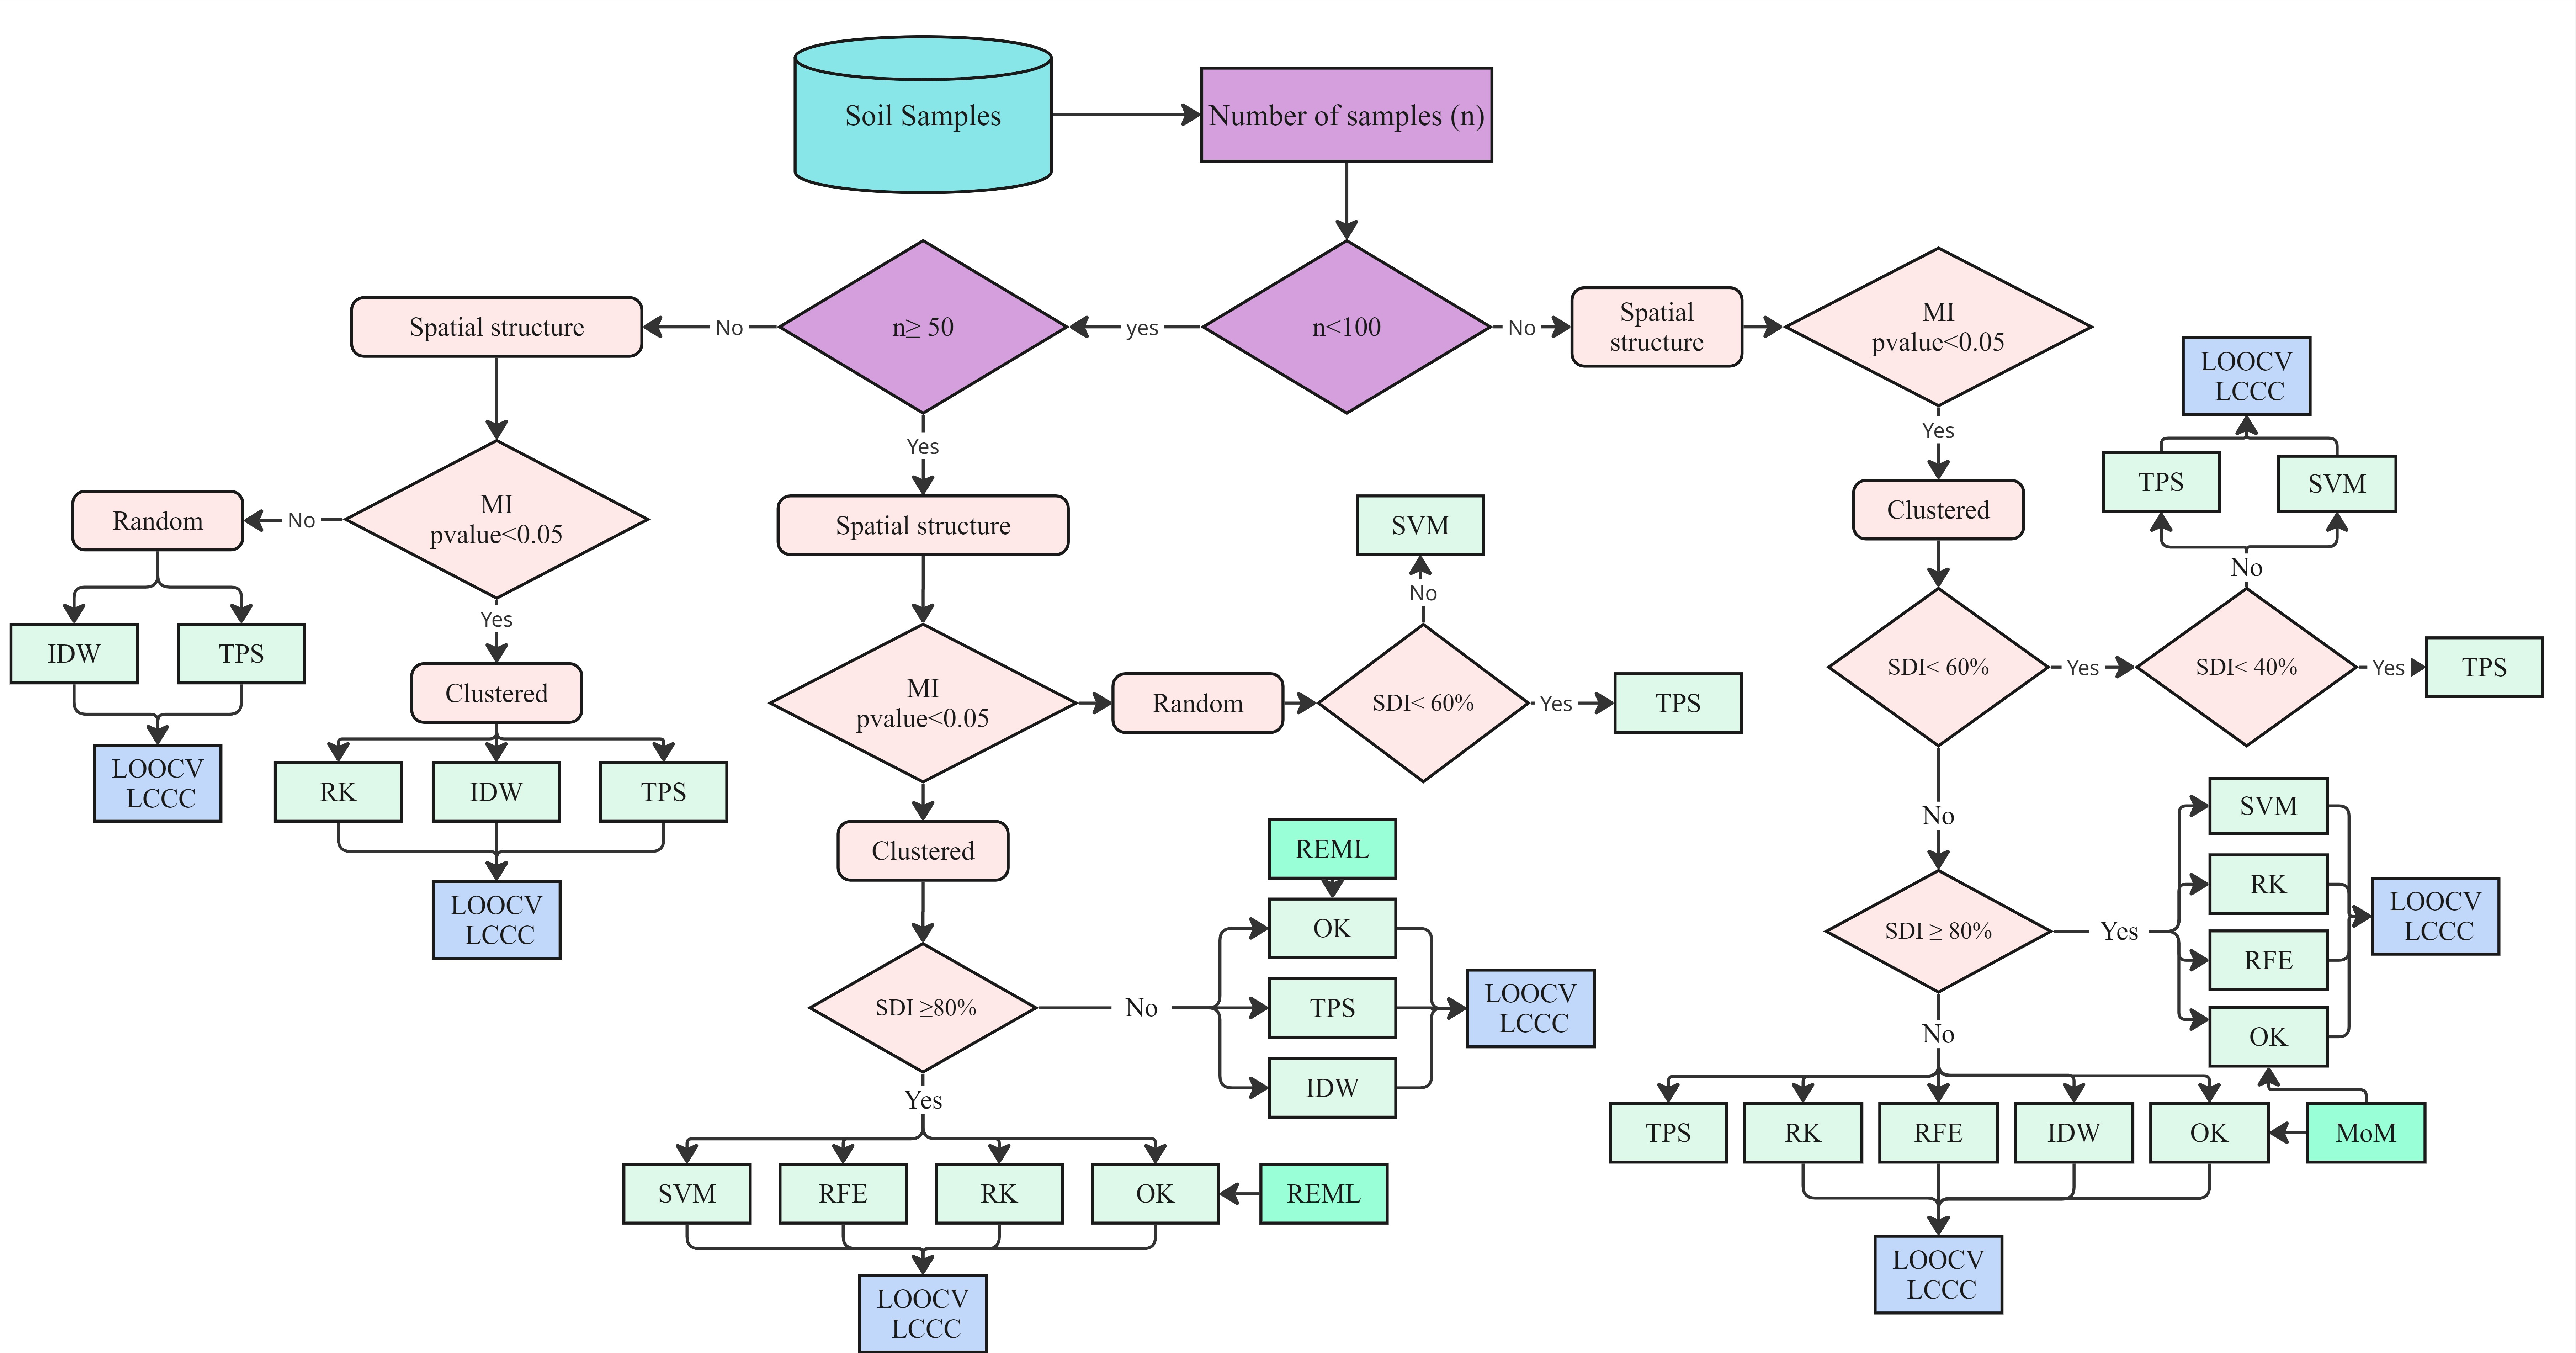
\includegraphics[width=0.95\textwidth]{multivariate_framework.png}
    \caption{Multivariate decision framework for interpolation method selection using auxiliary covariates.}
    \label{fig:multivariate_framework}
\end{figure}

% --------------------------------------------------
% Software requirements
% --------------------------------------------------

\section{Software Requirements}

The minimum declared QGIS version is \minimumqgisversion{}. The updated plugin supports the Qt 5 environment used by QGIS 3 and the Qt 6 environment used by QGIS 4. The same workflow is used across these environments; operating-system fonts, window borders, and individual QGIS controls may differ.

Compatibility checks cover each stable QGIS 3 minor series from 3.14 through 3.44, together with QGIS 4.0 and 4.2. Native Windows checks also cover QGIS 3.14 in 32-bit mode, QGIS 3.44.8 in 64-bit mode, and QGIS 4.2.3. Future releases are added to the compatibility checks as they become available; this is an ongoing verification process.

\begin{table}[H]
\centering
\caption{Software requirements and documentation scope.}
\begin{tabularx}{0.96\textwidth}{P{4.5cm}Y}
\toprule
\textbf{Component} & \textbf{Description} \\
\midrule
GIS software & QGIS 3.14 or later; QGIS 3 and 4 interfaces are supported \\
Python & Use the Python environment distributed with the installed QGIS \\
Machine learning & A compatible NumPy, SciPy, pandas, and scikit-learn stack in that QGIS environment \\
REML & The current implementation provides a Python/SciPy backend; a separate R installation is not a general prerequisite \\
Documentation & User guide for the current interface and analysis workflows \\
\bottomrule
\end{tabularx}
\end{table}

\begin{infobox}
The examples describe the updated interface. Older packaged releases may not include all of these controls. Record the installed plugin version from \texttt{About}, the QGIS version, and the operating system for reproducible work.
\end{infobox}

\section{Input Data Requirements}

The \textit{Best Fit Interpolator Plugin} requires spatial input data to perform interpolation, validation, and method recommendation. The minimum input data include a point layer containing sampled observations and a polygon layer defining the mapping area. Additional raster covariates can be used for multivariate interpolation methods.

The plugin was developed to support spatial mapping workflows based on point observations. These observations may represent soil attributes, environmental measurements, crop indicators, sensor-based variables, or other spatially distributed variables collected at known locations.

\subsection{Point Layer}

The point layer contains the sampled observations used as input for interpolation. Each point must have a valid geometry and an attribute table containing at least one numerical variable to be mapped.

\begin{table}[H]
\centering
\caption{Minimum requirements for the point layer.}
\begin{tabular}{P{5cm} P{8cm}}
\toprule
\textbf{Requirement} & \textbf{Description} \\
\midrule
Geometry type & Point layer \\
Coordinate reference system & Projected CRS recommended, preferably UTM \\
Attribute table & At least one numerical target variable \\
Missing values & Missing or invalid values should be removed before interpolation \\
Sampling locations & Points should be located inside or near the mapping boundary \\
\bottomrule
\end{tabular}
\end{table}

\begin{infobox}
The plugin uses the selected numerical field as the target variable for interpolation. Non-numerical fields should not be selected as interpolation variables.
\end{infobox}

\subsection{Boundary Polygon}

The boundary polygon defines the spatial extent of the interpolation. The interpolated raster is generated according to this area and should represent the region where spatial prediction is required.

\begin{table}[H]
\centering
\caption{Minimum requirements for the boundary polygon.}
\begin{tabular}{P{5cm} P{8cm}}
\toprule
\textbf{Requirement} & \textbf{Description} \\
\midrule
Geometry type & Polygon layer \\
Purpose & Defines the interpolation extent and output raster mask \\
Coordinate reference system & Same CRS as the point layer is recommended \\
Geometry validity & The polygon should be valid and free of topology errors \\
\bottomrule
\end{tabular}
\end{table}

\begin{infobox}
The boundary polygon is used to limit the spatial prediction area. It helps avoid generating maps outside the area of interest.
\end{infobox}

\subsection{Auxiliary Raster Covariates}

Auxiliary raster covariates are optional input layers that can be used in multivariate interpolation methods. These covariates should represent spatial information that may help explain the variability of the target variable.

Examples of auxiliary covariates include:

\begin{itemize}
    \item elevation or terrain attributes;
    \item apparent electrical conductivity;
    \item vegetation indices;
    \item bare soil indices;
    \item remote sensing products;
    \item proximal sensing layers;
    \item management or environmental layers.
\end{itemize}

\begin{infobox}
Auxiliary covariates are especially useful when they are spatially continuous and related to the target variable. Poorly related covariates may not improve interpolation performance.
\end{infobox}

\subsection{Coordinate Reference System}

Distance-based interpolation methods require reliable distance calculations. For this reason, the use of a projected coordinate reference system is strongly recommended.

Geographic coordinate systems, such as latitude and longitude, should be avoided for interpolation because distances are expressed in degrees rather than meters.

\begin{table}[H]
\centering
\caption{Recommended coordinate reference system configuration.}
\begin{tabular}{P{5cm} P{8cm}}
\toprule
\textbf{Layer} & \textbf{Recommendation} \\
\midrule
Point layer & Projected CRS, preferably UTM \\
Boundary polygon & Same CRS as the point layer \\
Raster covariates & Same CRS and compatible resolution when possible \\
QGIS project & Same projected CRS used by the input layers \\
\bottomrule
\end{tabular}
\end{table}

\begin{infobox}
Using different coordinate reference systems among point, polygon, and raster layers may cause misalignment, incorrect distance calculations, or failed interpolation outputs.
\end{infobox}

% --------------------------------------------------
% General workflow
% --------------------------------------------------

% --------------------------------------------------
% General workflow
% --------------------------------------------------
\section{General Workflow}


The \textit{Best Fit Interpolator Plugin} follows a shared preparation stage and then separates into two independent analysis paths. The user may run a manual interpolation workflow, choosing one or more deterministic, geostatistical, or machine learning methods, or may use the framework-guided workflow to obtain a method recommendation from the decision framework. These paths are not sequential requirements; the framework does not need to be run after the manual workflow, and the manual workflow does not need to be run before the framework.


\subsection{Shared Preparation}


Before choosing the analysis path, prepare the project and load the common inputs:


\begin{enumerate}
    \item Load the input layers in QGIS.
    \item Open the \textit{Best Fit Interpolator Plugin}.
    \item Select the point layer containing the sampled observations.
    \item Select the target variable to be interpolated.
    \item Select the boundary polygon that defines the mapping area.
    \item Define the output pixel size.
    \item Review the spatial diagnostics and the data preview.
\end{enumerate}


\subsection{Path A: Manual Interpolation}


Use this path when the user wants to choose and run a specific interpolation method directly.


\begin{enumerate}
    \item Select the interpolation family: deterministic, geostatistical, or machine learning.
    \item Configure the selected method and its parameters.
    \item For machine learning methods, load and prepare the covariate rasters before fitting the model.
    \item Run the interpolation.
    \item Evaluate the result using the validation metrics and diagnostic plots.
    \item Export the final raster and summary outputs.
\end{enumerate}


\subsection{Path B: Framework-Guided Recommendation}


Use this path when the user wants the plugin to support method selection using the decision framework. The framework uses the characteristics of the loaded data and the validation information available in the project to guide the recommendation. It is an independent workflow and should be interpreted as decision support rather than as a mandatory step after manual interpolation.


\begin{enumerate}
    \item Open the framework workflow after loading the common data inputs.
    \item Review the data characteristics and diagnostic information used by the framework.
    \item Generate the framework-based recommendation.
    \item Use the recommendation to decide which interpolation method should be run or reported.
    \item Export the framework summary when documentation of the decision process is required.
\end{enumerate}


\begin{infobox}
The plugin does not assume that one interpolation method is universally superior. Manual interpolation and framework-guided recommendation are complementary but independent workflows. The user may choose either path according to the objective of the mapping process.
\end{infobox}


\section{Installing the Plugin}

The \textit{Best Fit Interpolator Plugin} can be installed directly from the official QGIS Plugin Repository or from the ZIP package published on GitHub. Installation through the official repository is recommended for most users because QGIS can detect future updates automatically.

\begin{infobox}
Use the official QGIS repository whenever the plugin is publicly available. Use the GitHub ZIP method for a specific release, testing, or controlled installation. Do not extract the ZIP file before installing it in QGIS.
\end{infobox}

\subsection{Installation from the Official QGIS Plugin Repository}

\tutorialstep{Open the QGIS Plugin Manager}{
Start QGIS and open \textbf{Plugins $>$ Manage and Install Plugins}. QGIS will display the plugin manager and refresh the configured repositories.
}



\tutorialstep{Search for the plugin}{
Select \textbf{All} in the left panel and type \textbf{Best Fit Interpolator} in the search field. Select the plugin when it appears in the results.
}



\tutorialstep{Install the plugin}{
Review the plugin name, version, author, and description. Click \textbf{Install Plugin} and wait until QGIS confirms that the installation was completed successfully.
}



\tutorialstep{Verify the installation}{
Open the \textbf{Installed} tab and confirm that \textbf{Best Fit Interpolator} is listed and enabled. The plugin can then be opened from the QGIS plugin interface.
}



\subsection{Installation from a GitHub Release ZIP}

The verified release packages are published on the
\href{https://github.com/ladelgadobe/BestFitInterpolation/releases}{Best Fit Interpolator GitHub Releases page}.
Select the packaged plugin ZIP from the release assets. Its release identifier may change; the installation procedure and this manual's filename remain the same.

\tutorialstep{Download the release package}{
Open the GitHub Releases page, select the appropriate current release, and download the packaged plugin ZIP from the release assets. Keep the downloaded file compressed.
}



\tutorialstep{Open Install from ZIP}{
In QGIS, open \textbf{Plugins $>$ Manage and Install Plugins}, then select \textbf{Install from ZIP} in the left panel.
}



\tutorialstep{Select and install the ZIP}{
Use the browse button to select the packaged plugin ZIP downloaded from the release assets. Click \textbf{Install Plugin} and accept the QGIS confirmation only when the package was downloaded from the official project release.
}



\tutorialstep{Confirm that the plugin is enabled}{
After the success message appears, open the \textbf{Installed} tab and verify that the plugin is enabled. If another version was previously installed, restart QGIS before testing the updated plugin.
}



\subsection{GitHub Repository and Release History}

The public source code, documentation, issue tracker, tags, and releases are maintained at
\url{https://github.com/ladelgadobe/BestFitInterpolation}.
The repository is useful for reviewing the source code, reporting problems, and consulting version history. End users should install a packaged release ZIP rather than downloading the automatically generated \textit{Source code} archives, because those archives may contain development files that are not part of the QGIS installation package.

\begin{infobox}
For reproducible work, record the plugin version, QGIS version, operating system, and installation method used in the project.
\end{infobox}

\clearpage

% --------------------------------------------------
% Opening the plugin and interface overview
% --------------------------------------------------
\section{Opening the Plugin and Interface Overview}

Before loading data, the QGIS project must be saved. This requirement gives the plugin a stable working location for the output folder, rasters, validation products, and reports created during the analysis.

\tutorialstep{Locate the plugin in QGIS}{
Open \texttt{Plugins > Best Fit Interpolator > Best Fit Interpolator}. The plugin can also be opened by clicking its icon on the QGIS toolbar.
}



\tutorialstep{Save the QGIS project}{
If the current QGIS project has not been saved, the plugin displays the message \textit{Project must be saved}. Click \texttt{OK}, select \texttt{Project > Save As}, choose a suitable working folder, and save the project as a \texttt{.qgz} file.
}



\begin{infobox}
The output folder is created next to the saved QGIS project file. Use a descriptive project name and a working directory where the user has permission to create and modify files.
\end{infobox}

\tutorialstep{Open the plugin again}{
After saving the project, open Best Fit Interpolator again from the Plugins menu or toolbar. The main window opens on the \texttt{Data} tab with a fresh session. Closing and reopening resets selections, diagnostic decisions, validation results, previews, and the Framework result. Export the outputs and record sample decisions before closing if they must be retained. The \texttt{About} tab provides the installed version, authors, manual, reference article, GitHub repository, support links, and the authors' LinkedIn profiles.
}

\begin{figure}[H]
    \centering
    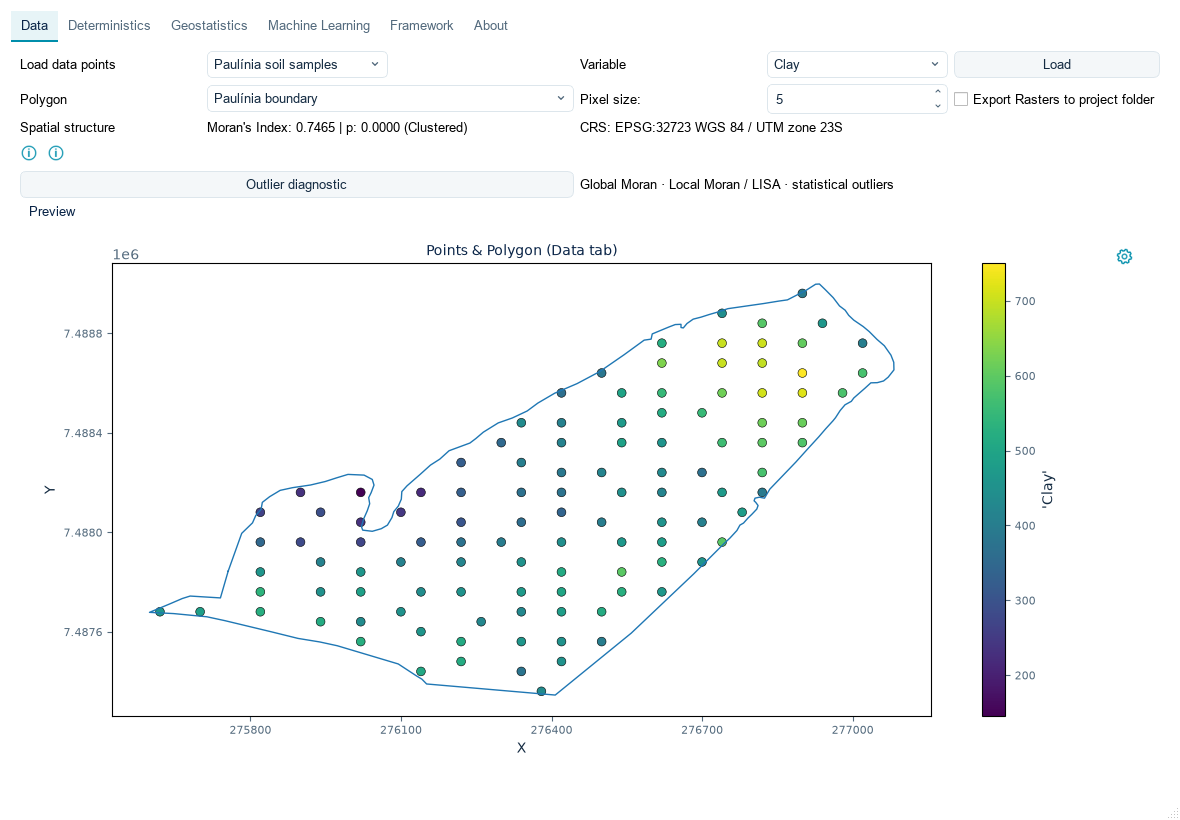
\includegraphics[width=0.94\textwidth,height=0.66\textheight,keepaspectratio]{data.png}
    \caption{Data tab after loading the core inputs, with the common input controls and the Outlier diagnostic entry point.}
    \label{fig:main-interface-data}
\end{figure}

% --------------------------------------------------
% Loading core data
% --------------------------------------------------

\begin{figure}[H]
    \centering
    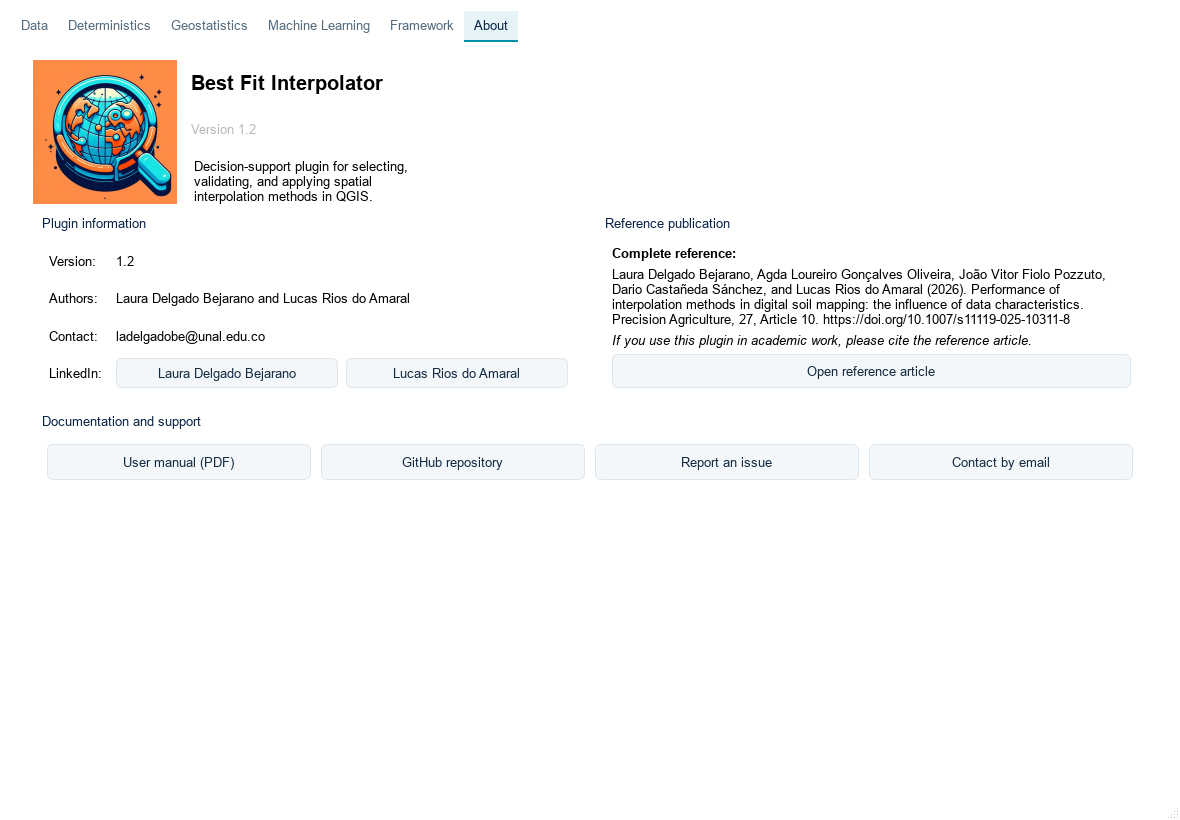
\includegraphics[width=0.97\textwidth,height=0.60\textheight,keepaspectratio]{about.png}
    \caption{About page with the plugin identity, installed version, manual, article, and support links.}
    \label{fig:about}
\end{figure}

\section{Loading Core Data}

The \texttt{Data} tab defines the common configuration shared by both independent workflows: manual interpolation and framework guidance. Before starting, load the point and polygon layers into the QGIS project. Figure~\ref{fig:main-interface-data} shows the common inputs to review before analysis.

\subsection{Common Data Controls}

\begin{enumerate}
    \item \textbf{Load data points.} Select the point layer containing the sampled observations. The list is populated from point layers already loaded in the current QGIS project. Each point must have valid geometry and a usable value in the target attribute.

    \item \textbf{Polygon.} Select the polygon layer that defines the study area, interpolation extent, and output mask. The polygon must be valid, loaded in QGIS, and expressed in the same projected metric CRS as the point layer.

    \item \textbf{Variable and Load.} Select the numerical attribute to interpolate. The variable list is updated from the fields of the selected point layer. After selecting the point layer, polygon, and variable, click \texttt{Load}. The plugin filters incomplete or non-numerical values, calculates the spatial structure, displays the point-layer CRS, and creates the preview.

    \item \textbf{Pixel size.} Enter the output raster cell size in the units of the point-layer CRS. The value entered defines the dimensions of each output pixel. For example, when the CRS uses meters, entering \texttt{5} creates pixels measuring 5~m by 5~m. Smaller values produce a finer grid but increase processing time, memory use, and output file size.

    \item \textbf{Export Rasters to project folder.} Enable this option to save generated rasters in the \texttt{BestFitInterpolation} folder created beside the saved QGIS project. When it is disabled, raster outputs are temporary and should be exported manually before closing QGIS if they must be preserved.
\end{enumerate}

\subsection{Spatial Structure and Moran's Index}

After \texttt{Load} is clicked, the \texttt{Spatial structure} line reports Moran's Index, its p-value, and one of three spatial-pattern classes:

\begin{description}
    \item[Clustered:] nearby observations tend to have similar values, providing evidence of positive spatial autocorrelation.
    \item[Dispersed:] neighboring observations tend to be more dissimilar than expected under spatial randomness, providing evidence of negative spatial autocorrelation.
    \item[Random:] the observed spatial arrangement does not provide sufficient evidence of either clustering or dispersion.
\end{description}

The plugin calculates global Moran's I using a K-nearest-neighbor spatial structure with eight neighbors, row-standardized binary weights, and a permutation-based reference distribution. The displayed p-value indicates whether the observed pattern is statistically different from spatial randomness. The final class combines the direction of Moran's I with this statistical significance: \textit{Clustered} indicates significant positive spatial autocorrelation, \textit{Dispersed} indicates significant negative spatial autocorrelation, and \textit{Random} is used when the evidence is not strong enough to support either pattern.

For this reason, users should not interpret the sign of Moran's I alone. A positive or negative value only defines the direction of the pattern; the p-value determines whether that pattern is significant enough to guide the interpretation.


\subsection{Outlier Diagnostic}
\label{sec:outlier-diagnostic}

Click \texttt{Outlier diagnostic} in \texttt{Data} to review unusually large or small values and local spatial patterns before interpolation. The window combines statistical flags, Global Moran's I, Local Moran / LISA, a point map, histogram, boxplot, and a table. Click its information icon to open a readable help window that stays open while reviewing the definitions.


\begin{figure}[H]
    \centering
    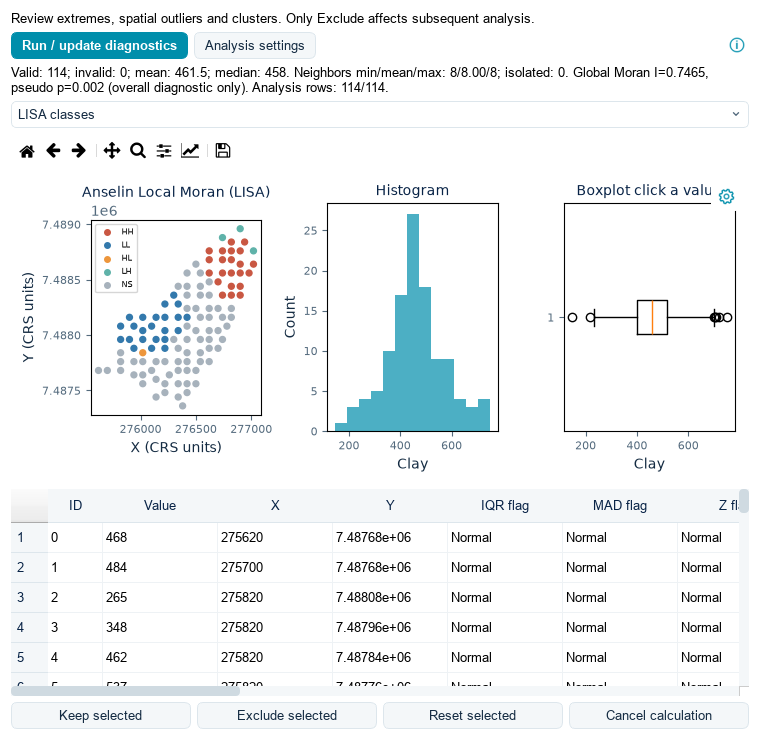
\includegraphics[width=0.97\textwidth,height=0.60\textheight,keepaspectratio]{outlier_diagnostic.png}
    \caption{Outlier diagnostic: linked map, distribution plots, feature table, and explicit sample decisions.}
    \label{fig:outlier-diagnostic}
\end{figure}

\subsubsection{Statistical Flags}

Statistical flags assess a value relative to the overall distribution. IQR and MAD are selected by default; classical Z is optional and is less robust to extreme observations.

\begin{itemize}
    \item \textbf{IQR.} With $\mathrm{IQR}=Q_3-Q_1$, values below $Q_1-k\,\mathrm{IQR}$ or above $Q_3+k\,\mathrm{IQR}$ are flagged. The default Tukey multiplier is $k=1.5$.
    \item \textbf{MAD.} The modified score is $0.67449(x-\mathrm{median})/\mathrm{MAD}$, where $\mathrm{MAD}=\mathrm{median}(|x-\mathrm{median}|)$. The default threshold is $|\mathrm{score}|>3.5$. If MAD is zero, values equal to the median score zero; unequal values receive signed infinity and require review.
    \item \textbf{Z.} The classical score uses the mean and standard deviation. Its default threshold is $|Z|>3$.
    \item \textbf{Statistical consensus.} \texttt{Any} flags a point if any selected method flags it. \texttt{All} requires all selected methods. \texttt{At least N} requires the chosen minimum number of flags. These settings combine statistical methods; spatial evidence is reported separately.
\end{itemize}

\subsubsection{Global and Local Spatial Evidence}

Global Moran's I describes the overall spatial pattern. It does not identify an individual point as an outlier. Local Moran / LISA evaluates each point relative to its neighbors, following the local association approach of \citet{anselin1995}. With centered values $z_i=x_i-\bar{x}$, the local statistic is
\[
 I_i=\frac{z_i}{m_2}\sum_j w_{ij}z_j,
 \qquad m_2=\frac{1}{n}\sum_i z_i^2.
\]
The plugin uses row-standardized binary neighborhood weights and conditional permutations that keep the focal value fixed while sampling possible neighbors from the other observations.

\begin{table}[H]
\centering
\caption{Reading Local Moran / LISA classes. H and L mean above and below the analysis mean.}
\label{tab:lisa-classes}
\begin{tabularx}{0.96\textwidth}{P{1.3cm}P{4.3cm}Y}
\toprule
\textbf{Class} & \textbf{Point and neighborhood} & \textbf{Interpretation} \\
\midrule
HH & High point, high neighbors & Significant cluster of high values \\
LL & Low point, low neighbors & Significant cluster of low values \\
HL & High point, low neighbors & Potential spatial outlier \\
LH & Low point, high neighbors & Potential spatial outlier \\
NS & No significant local pattern & Insufficient local evidence at the chosen alpha; statistical flags may still apply \\
Invalid & Unusable value or geometry & Cannot contribute to the analysis \\
\bottomrule
\end{tabularx}
\end{table}

The first letter describes the point and the second the mean of its neighbors. HH and LL are clusters, whereas HL and LH are the spatial-outlier classes. A significant local contrast may represent a genuine boundary, management effect, or environmental transition; it is not automatically a measurement error.

\subsubsection{Analysis Settings}

Click \texttt{Analysis settings} to open the parameter window. The statistical controls identify unusually large or small values; the neighborhood and LISA controls assess local spatial patterns. Table~\ref{tab:outlier-parameters} explains every control shown in Figure~\ref{fig:outlier-settings}.


\begin{figure}[H]
    \centering
    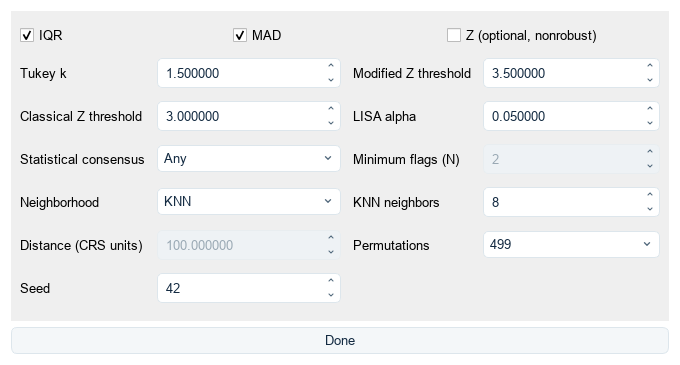
\includegraphics[width=0.85\textwidth,height=0.42\textheight,keepaspectratio]{outlier_settings.png}
    \caption{Analysis settings for statistical thresholds, consensus, neighborhood, permutations, alpha, and seed.}
    \label{fig:outlier-settings}
\end{figure}

\begin{longtable}{P{0.24\textwidth}P{0.12\textwidth}P{0.55\textwidth}}
\caption{Outlier diagnostic parameters and their interpretation.}\label{tab:outlier-parameters}\\
\toprule
\textbf{Control} & \textbf{Default} & \textbf{Meaning and use} \\
\midrule
\endfirsthead
\toprule
\textbf{Control} & \textbf{Default} & \textbf{Meaning and use} \\
\midrule
\endhead
\texttt{IQR}, \texttt{MAD}, \texttt{Z} & IQR and MAD & Select which statistical methods contribute to the consensus. Z is optional and nonrobust. These checkboxes do not turn LISA on or off. \\
\texttt{Tukey k} & 1.5 & Multiplier of the interquartile range in the IQR limits $Q_1-k\,\mathrm{IQR}$ and $Q_3+k\,\mathrm{IQR}$. Larger $k$ widens the limits and flags fewer values; smaller $k$ flags more. \\
\texttt{Modified Z threshold} & 3.5 & Absolute-score cutoff for MAD, using the median and median absolute deviation. A value is flagged when its modified score exceeds this cutoff in magnitude. A higher cutoff flags fewer values. \\
\texttt{Classical Z threshold} & 3.0 & Absolute-score cutoff for the optional Z method: $Z=(x-\mathrm{mean})/\mathrm{standard\ deviation}$. Unlike MAD, it uses the mean and standard deviation, which extreme values can distort. A higher cutoff flags fewer values. \\
\texttt{LISA alpha} & 0.05 & Maximum local pseudo p-value accepted as significant. Lower alpha requires stronger evidence; higher alpha accepts weaker evidence. It controls LISA classes, independently of the statistical thresholds. \\
\texttt{Statistical consensus} & Any & \texttt{Any}: at least one selected method must flag the point. \texttt{All}: every selected method must flag it. \texttt{At least N}: require a specified number of selected methods. \\
\texttt{Minimum flags (N)} & 2 & Active only with \texttt{At least N}. With IQR and MAD selected, $N=2$ requires both flags. Choose $N$ no larger than the number of selected methods; otherwise no point can meet the consensus. \\
\texttt{Neighborhood} & KNN & Choose \texttt{KNN} for a fixed neighbor count, or \texttt{Distance threshold} for a fixed radius. This changes the spatial context used by Global Moran and LISA. \\
\texttt{KNN neighbors} & 8 & Number of nearest other points used in KNN mode, limited by the available observations. Smaller counts emphasize local structure; larger counts represent a broader neighborhood. \\
\texttt{Distance (CRS units)} & 100 & Radius used only in \texttt{Distance threshold} mode. In a metric CRS, 100 means 100~m. A small radius can leave points isolated; check the isolated count before interpreting LISA. \\
\texttt{Permutations} & 499 & Random rearrangements used for the significance test; choices are 99, 499, and 999. More permutations improve pseudo p-value resolution and take longer. The minimum possible pseudo p-value is $1/(P+1)$. \\
\texttt{Seed} & 42 & Initializes the random generator. Keep the same inputs, neighborhood, permutations, and seed to reproduce a diagnostic run. Changing the seed can change the estimated pseudo p-values. \\
\texttt{Done} & & Closes the settings window. Return to the diagnostic window and click \texttt{Run / update diagnostics} to calculate results using the new settings. \\
\bottomrule
\end{longtable}

Start with the defaults, inspect the flags and neighboring values, and then adjust a parameter only when its interpretation fits the sampling design. Changing a threshold changes a diagnostic label; it does not establish that a measurement is wrong or automatically exclude it.

\begin{infobox}
Local pseudo p-values are not adjusted for multiple comparisons. Use the map and table as an exploratory diagnostic and interpret the evidence with sampling design and field knowledge. The configurable Global Moran result in this window may differ from the automatic \texttt{Data} summary because its neighborhood, seed, and permutation settings can differ.
\end{infobox}

\subsubsection{Reviewing and Applying Sample Decisions}

\begin{enumerate}
    \item Load the common inputs in \texttt{Data} and open \texttt{Outlier diagnostic}.
    \item Review \texttt{Analysis settings}, then click \texttt{Run / update diagnostics}. Inspect the valid count, missing values, neighbor counts, and isolated points.
    \item Switch between \texttt{LISA classes} and \texttt{Target values}. Select rows or points to link the table, map, and QGIS feature selection; the distribution plots provide another way to inspect extreme values.
    \item Check the original record, field notes, units, and neighboring measurements before deciding. For example, an HL point with an IQR flag deserves inspection, while an HH cluster may describe a real high-value zone.
    \item Use \texttt{Keep selected} to record retention, \texttt{Exclude selected} to omit the selected usable points from subsequent analysis, or \texttt{Reset selected} to clear the decision. Only Exclude changes the analysis mask; flags alone do not exclude points.
    \item Recalculate the diagnostics and rerun fitting, validation, interpolation, and comparisons as needed after changing the analysis population. Review the updated sample count before accepting results.
\end{enumerate}

The original point layer is preserved. Keep cannot make invalid values or missing geometries usable. Decisions belong to the selected layer and target variable within the current plugin session; record the feature IDs and reasons before closing. Changing the data invalidates diagnostic and model snapshots so that an earlier result is not silently reused.


\subsection{Coordinate Reference System}

The \texttt{CRS} line displays the coordinate reference system of the selected point layer. The CRS is not configured or transformed inside the plugin. Input layers must be prepared in QGIS before loading them.

\begin{infobox}
Use a projected CRS whose map units are meters, such as the appropriate local UTM zone. Do not use a geographic latitude--longitude CRS such as EPSG:4326. Geographic coordinates are expressed in degrees, so distance calculations, Moran's Index, pixel size, and distance-based interpolation can fail or produce incorrect results. Reproject the point and polygon layers to the same metric CRS before continuing.
\end{infobox}

If the selected point layer does not use meter units, the plugin displays the warning \textit{Metric CRS required}. The plugin also checks whether the point and polygon layers use compatible CRSs and whether valid sample points overlap the selected polygon. A warning is shown in the \texttt{Data} tab, and interpolation is blocked if the spatial inputs are incompatible or if no usable samples fall inside the polygon. Resolve these problems before running interpolation or validation.

\subsection{Preview}

The preview displays the sample points colored according to the selected variable together with the boundary polygon. Use it to verify that the correct layers and variable were selected, that the samples fall within the intended study area, and that the spatial distribution and value range appear reasonable.



% --------------------------------------------------
% Deterministic interpolation
% --------------------------------------------------
\section{Deterministic Interpolation: IDW and TPS}

After the common inputs have been loaded in the \texttt{Data} tab, open \texttt{Deterministics}. This tab provides three mutually exclusive interpolation choices: Inverse Distance Weighting (IDW) with manual parameters, IDW with automatic optimization, and Thin Plate Spline (TPS). At least ten valid observations are required to run an interpolation.

\begin{figure}[H]
    \centering
    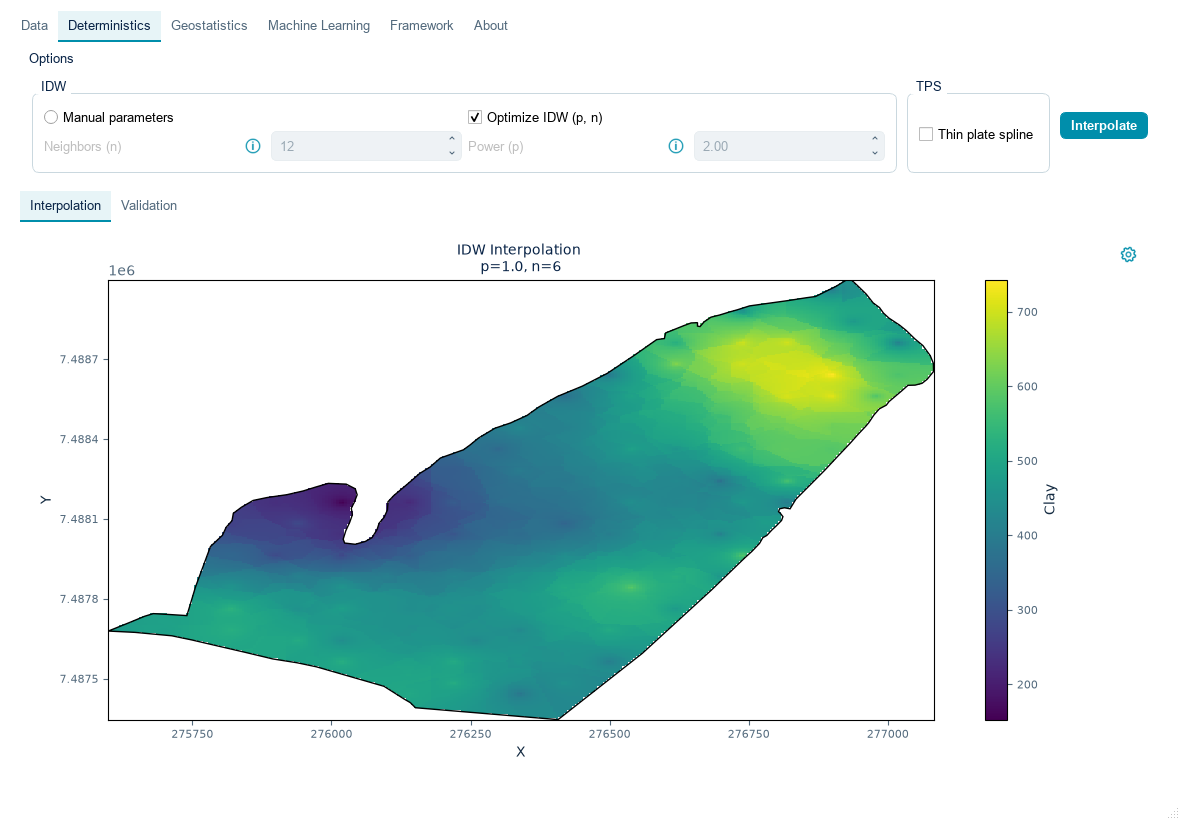
\includegraphics[width=0.94\textwidth,height=0.68\textheight,keepaspectratio]{deterministics.png}
    \caption{Deterministics tab showing the available interpolation methods and the result window for the selected method.}
    \label{fig:deterministics-interpolation}
\end{figure}

\subsection{Available Interpolation Options}

\begin{enumerate}
    \item \textbf{Manual IDW.} Select \texttt{Manual parameters}, then enter the neighbor count $n$ and power $p$. The neighbor count controls the observations used for each prediction. Smaller neighborhoods emphasize local variation; larger neighborhoods generally produce smoother surfaces. Increasing $p$ gives nearby observations more influence. Decreasing $p$ spreads influence across the neighborhood.


    \item \textbf{Optimized IDW.} Select \texttt{Optimize IDW (p, n)} when the plugin should choose both parameters automatically. The manual $p$ and $n$ controls are disabled in this mode. The plugin evaluates candidate $p$ and $n$ combinations using five-fold cross-validation and selects the combination with the smallest Interpolation Selection Index (ISI), which combines normalized mean absolute error and the variability of prediction errors \citep{bierdesouza2017}.


    \item \textbf{Thin Plate Spline (TPS).} Select \texttt{Thin plate spline} to create a smooth surface using a radial-basis thin-plate spline. TPS does not expose additional parameters in this tab. For normal datasets it uses the global thin-plate spline. Dense and massive profiles use a local neighborhood, as described in Section~\ref{sec:dense-massive}. It requires unique sampling coordinates; duplicate point coordinates must be resolved before interpolation.




    \item \textbf{Run the selected method.} Click \texttt{Interpolate}. The plugin reuses the point layer, target variable, polygon, pixel size, and export option defined in the \texttt{Data} tab. The resulting surface is shown in the \texttt{Interpolation} subtab, clipped to the selected polygon, and added to QGIS. When raster export is enabled, the file is also written to the project output folder.
\end{enumerate}

\begin{infobox}
Manual IDW, optimized IDW, and TPS cannot run simultaneously. Selecting one option automatically deactivates the others. The displayed interpolation map is a visual result; method performance must be assessed in the \texttt{Validation} subtab using the same configuration that produced the interpolation.
\end{infobox}



% --------------------------------------------------
% Ordinary Kriging
% --------------------------------------------------
\section{Ordinary Kriging: MoM and REML}

After loading the common inputs, open the \texttt{Geostatistics} tab. The plugin applies Ordinary Kriging and provides two approaches for estimating the semivariogram or covariance parameters: the Method of Moments (MoM) and Residual Maximum Likelihood (REML). The interpolated surface is always produced for the same variable, polygon, pixel size, and export configuration loaded in the \texttt{Data} tab.

\subsection{Automatic Choice Between MoM and REML}

When \texttt{Fit method} is set to \texttt{Automatic}, the plugin uses REML for fewer than 100 valid samples when the REML backend is available, and MoM for 100 samples or more. This implementation rule is consistent with the sampling evidence discussed by \citet{kerryoliver2007}: empirical semivariograms calculated by MoM commonly require approximately 100 appropriately spaced observations, whereas REML can provide useful parameter estimates with smaller samples. The threshold is a practical plugin rule, not a universal statistical boundary; sampling design, spatial structure, and data quality still matter.

The user can override the automatic choice by selecting \texttt{MoM} or \texttt{REML}. Manual REML is available for datasets with fewer than 500 valid samples. For 500 samples or more, the plugin uses MoM because REML optimization can become computationally expensive.

\subsection{Method of Moments  (MoM)}

Figure~\ref{fig:geostatistics-mom} shows the MoM workspace: experimental semivariogram, fitted theoretical model, spatial-dependence summary, and resulting Ordinary Kriging map.

\begin{figure}[H]
    \centering
    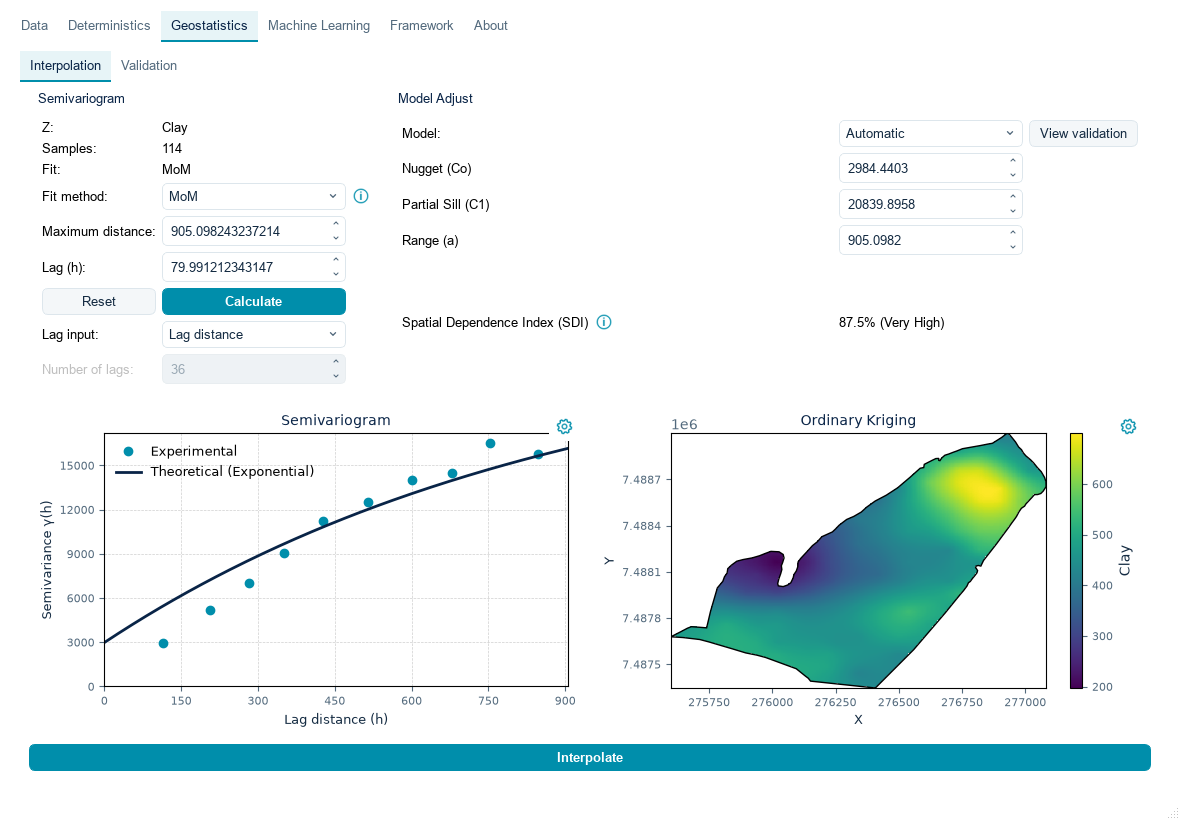
\includegraphics[width=0.96\textwidth,height=0.72\textheight,keepaspectratio]{geostatistics_mom.png}
    \caption{Geostatistics tab using MoM with an experimental semivariogram, a fitted theoretical model, the Spatial Dependence Index, and the Ordinary Kriging map.}
    \label{fig:geostatistics-mom}
\end{figure}

The \texttt{Semivariogram} panel reports the target variable (\texttt{Z}), number of valid samples, and selected fitting method. \texttt{Maximum distance} defines the greatest point-pair separation used to construct the experimental semivariogram, while \texttt{Lag (h)} defines the distance-class width. Click \texttt{Calculate} after changing either value. \texttt{Reset} restores the automatically proposed configuration.

Under \texttt{Model Adjust}, the plugin can evaluate three theoretical semivariogram models:

\begin{itemize}
    \item \textbf{Spherical:} increases with distance and reaches its sill at the specified range.
    \item \textbf{Exponential:} approaches the sill progressively and can represent spatial correlation that decays gradually.
    \item \textbf{Gaussian:} is smooth near the origin and is suitable when short-distance variation changes gradually.
\end{itemize}

With \texttt{Model} set to \texttt{Automatic}, the plugin evaluates the Spherical, Exponential, and Gaussian models by leave-one-out cross-validation. In Geostatistics, it ranks the candidates by the highest Lin's concordance correlation coefficient (LCCC), then the lowest root mean square error (RMSE), and then the highest $R^2$ if a further tie remains. Click \texttt{View validation} to inspect RMSE, RMSE\%, MAE, $R^2$, Pearson correlation, and Lin's concordance correlation coefficient for the three candidate models. Select a successful model row when another candidate is preferable. The Framework semivariogram popup uses its own $R^2$/RMSE ranking, described later in this manual.

The model can also be selected manually. The user may adjust \texttt{Nugget (C0)}, \texttt{Partial Sill (C1)}, and \texttt{Range (a)} before interpolating. The nugget represents unresolved short-range variation and measurement error; the partial sill represents the spatially structured variance; and the range indicates the distance over which spatial dependence is expressed. Manual values should be used only when they are supported by the experimental semivariogram and subject-matter knowledge.

The blue points in the left plot are the experimental semivariances calculated from sample pairs, and the black curve is the fitted theoretical model. The right plot previews the Ordinary Kriging surface inside the selected polygon. After reviewing the model, click \texttt{Interpolate} to create the final raster.

\subsection{Spatial Dependence Index}

The plugin calculates the Spatial Dependence Index (SDI) from the fitted nugget and partial sill:

\[
    \mathrm{SDI}=\frac{C1}{C0+C1}\times 100\%.
\]

\begin{table}[H]
    \centering
    \caption{Spatial Dependence Index classification used by the plugin.}
    \label{tab:sdi-classification}
    \begin{tabular}{ll}
        \toprule
        \textbf{SDI (\%)} & \textbf{Classification} \\
        \midrule
        $0 \leq \mathrm{SDI} < 20$ & Very Low \\
        $20 \leq \mathrm{SDI} < 40$ & Low \\
        $40 \leq \mathrm{SDI} < 60$ & Moderate \\
        $60 \leq \mathrm{SDI} < 80$ & High \\
        $80 \leq \mathrm{SDI} \leq 100$ & Very High \\
        \bottomrule
    \end{tabular}
\end{table}

A low SDI indicates that the nugget accounts for a large share of the total fitted variance. A high SDI indicates that the spatially structured component is dominant. SDI describes the fitted spatial-dependence structure; it is not, by itself, a measure of predictive accuracy. In Figure~\ref{fig:geostatistics-mom}, the displayed SDI describes this teaching dataset and should be read from the current fitted parameters.

\subsection{Residual Maximum Likelihood (REML)}

REML estimates the covariance parameters by maximizing a residual likelihood rather than first calculating and fitting experimental semivariogram points. Consequently, the REML view does not display an experimental semivariogram. It reports the estimated model parameters and uses them directly for Ordinary Kriging.

REML can be advantageous for smaller datasets because it accounts for parameter estimation through a likelihood-based procedure, but its numerical optimization is more demanding than MoM. For this reason, the plugin recommends REML automatically only below 100 valid samples when its backend is available, permits manual REML below 500 samples, and avoids it for larger datasets.

\begin{infobox}
The \texttt{View validation} button compares theoretical semivariogram models using the current fitting method. REML shows only a theoretical curve; changing between MoM and REML refreshes the corresponding view. It is different from the common \texttt{Validation} subtab used later to evaluate the predictive performance of the completed interpolation.
\end{infobox}

\begin{figure}[H]
    \centering
    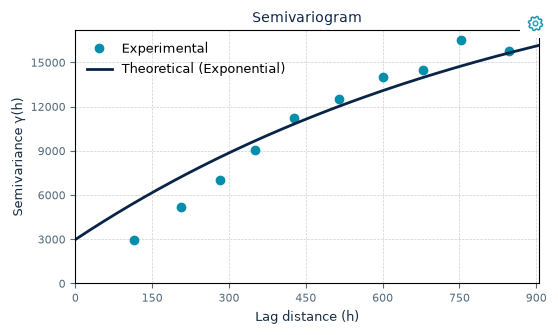
\includegraphics[width=0.84\textwidth,height=0.35\textheight,keepaspectratio]{semivariogram_mom.png}
    \caption{MoM view: experimental semivariances and fitted theoretical curve.}
    \label{fig:mom-curve}
\end{figure}

\begin{figure}[H]
    \centering
    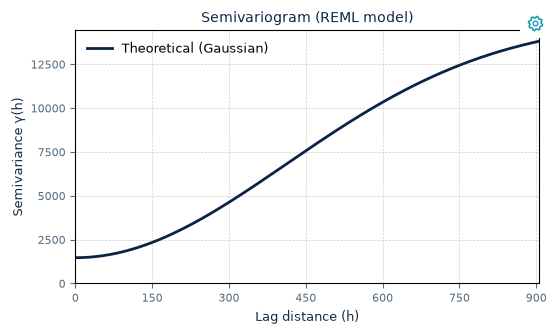
\includegraphics[width=0.84\textwidth,height=0.35\textheight,keepaspectratio]{semivariogram_reml.png}
    \caption{REML view: theoretical model only; no experimental semivariogram is displayed.}
    \label{fig:reml-curve}
\end{figure}


% --------------------------------------------------
% Machine learning interpolation
% --------------------------------------------------
\section{Machine Learning Interpolation}


After the common inputs have been loaded in the \texttt{Data} tab, open the \texttt{Machine Learning} tab when the interpolation should use environmental predictors in addition to the sampled target variable. In this workflow, the point observations provide the response values, while raster covariates provide predictor variables that help explain spatial variation across the study area. These covariate rasters must first be loaded in the QGIS project environment; the plugin reads the raster layers available in QGIS and does not create or download covariates automatically.


\subsection{Covariates}
\label{sec:ml-covariates}


Covariates are raster layers that describe auxiliary spatial information related to the target variable. Examples may include elevation, terrain derivatives, spectral indices, soil maps, climate layers, or any other continuous raster predictor prepared by the user. Because the plugin works inside QGIS, the covariate rasters should be added to the QGIS layer panel before they are selected in the \texttt{Machine Learning} tab.


Figure~\ref{fig:ml-covariates} shows the covariates window used before fitting machine learning models. The same tab brings together raster loading, covariate preprocessing, resampling, standardization, extraction of raster values to sample points, and correlation diagnostics.


\begin{figure}[H]
    \centering
    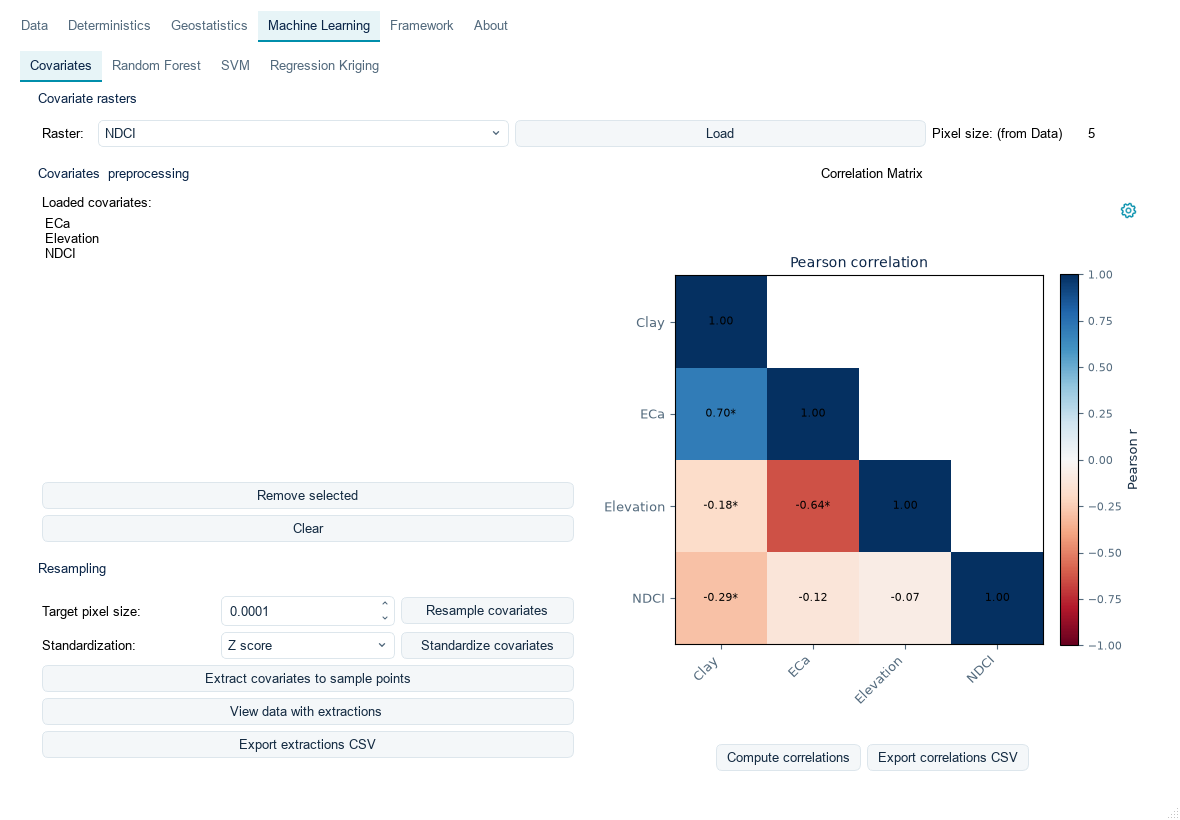
\includegraphics[width=0.94\textwidth,height=0.68\textheight,keepaspectratio]{covariates.png}
    \caption{Machine Learning covariates tab showing raster loading, covariate preprocessing, resampling, standardization, extraction controls, and the Pearson correlation matrix.}
    \label{fig:ml-covariates}
\end{figure}


\begin{enumerate}
    \item \textbf{Load covariate rasters.} Select each raster layer from the QGIS project and click \texttt{Load}. The loaded-covariates list is updated as rasters are added, removed, cleared, resampled, or standardized.


    \item \textbf{Check spatial compatibility.} Covariates should use the same projected CRS as the point and polygon layers. They should also have compatible extent, resolution, and alignment so that the value extracted at each sample point represents the same spatial support.


    \item \textbf{Resample covariates when needed.} Use \texttt{Resample covariates} when the raster predictors have different pixel sizes, extents, or grid alignment. The target pixel size can follow the output pixel size defined in the \texttt{Data} tab or another value selected by the user in the covariates window. Resampling creates a consistent predictor stack, so each grid cell used for interpolation is described by covariate values with the same spatial support.


    \item \textbf{Standardize covariates when appropriate.} The \texttt{Standardization} control provides two options: \texttt{Z-score} and \texttt{Range [-1,1]}. \texttt{Z-score} centers each covariate and expresses values relative to its variability, while \texttt{Range [-1,1]} rescales values to a common interval from -1 to 1. These transformations help place covariates with different units and numerical ranges on comparable scales, which is especially useful for scale-sensitive models such as Support Vector Machine.


    \item \textbf{Extract covariates to sample points.} After the covariates are prepared, extract their raster values at the sampled point locations. These extracted values form the predictor table used to train the machine learning models.


    \item \textbf{Review covariate correlations.} Use the correlation matrix as a diagnostic tool to inspect relationships among the target variable and the selected covariates. Strong correlations between covariates may indicate redundant predictors, while weak relationships with the target variable may reduce model usefulness.
\end{enumerate}


\begin{infobox}
Machine learning interpolation depends strongly on covariate quality. Covariates with missing values, mismatched CRS, incomplete coverage, weak relationship with the target variable, or excessive redundancy can reduce model performance even when the algorithm runs successfully.
\end{infobox}


\subsection{Available Machine Learning Methods}


The plugin includes Random Forest, Support Vector Machine (SVM), and Regression Kriging workflows. The following model-specific items describe the parameters available in the interface, the validation controls, and the expected outputs.


\begin{infobox}
The first time the plugin is installed, or the first time a machine learning method such as RF or SVM is executed in a QGIS environment without the required Python packages, the plugin may request permission to install the missing machine learning dependencies automatically. This step prepares the QGIS Python environment for methods that use \texttt{scikit-learn}. After the dependencies are available, the same installation prompt should not appear again for that environment.
\end{infobox}


\subsubsection{Random Forest}


In the plugin, Random Forest (RF) is implemented as a spatial machine learning interpolation method. The model can use the point coordinates, represented by \texttt{x} and \texttt{y}, together with the raster covariates loaded in the \texttt{Covariates} tab. In this way, RF can learn from both the spatial position of the samples and the environmental predictors prepared in QGIS.


Before running RF, complete the \texttt{Covariates} workflow: load the predictor rasters, resample or standardize them when needed, and extract covariate values to the sample points. When RF interpolation or RF hyperparameter search starts, the plugin opens a predictor-selection dialog. This dialog allows the user to choose the final variables that will be used by the model, including \texttt{x}, \texttt{y}, and any loaded raster covariates. Only the selected predictors are used for training, hyperparameter search, and map prediction.


Figure~\ref{fig:rf-interpolation} shows the RF interpolation window. The upper panel contains the manual and Grid Search controls, while the lower panels show the variable-importance plot and the RF interpolation map produced after the model is fitted.


\begin{figure}[H]
    \centering
    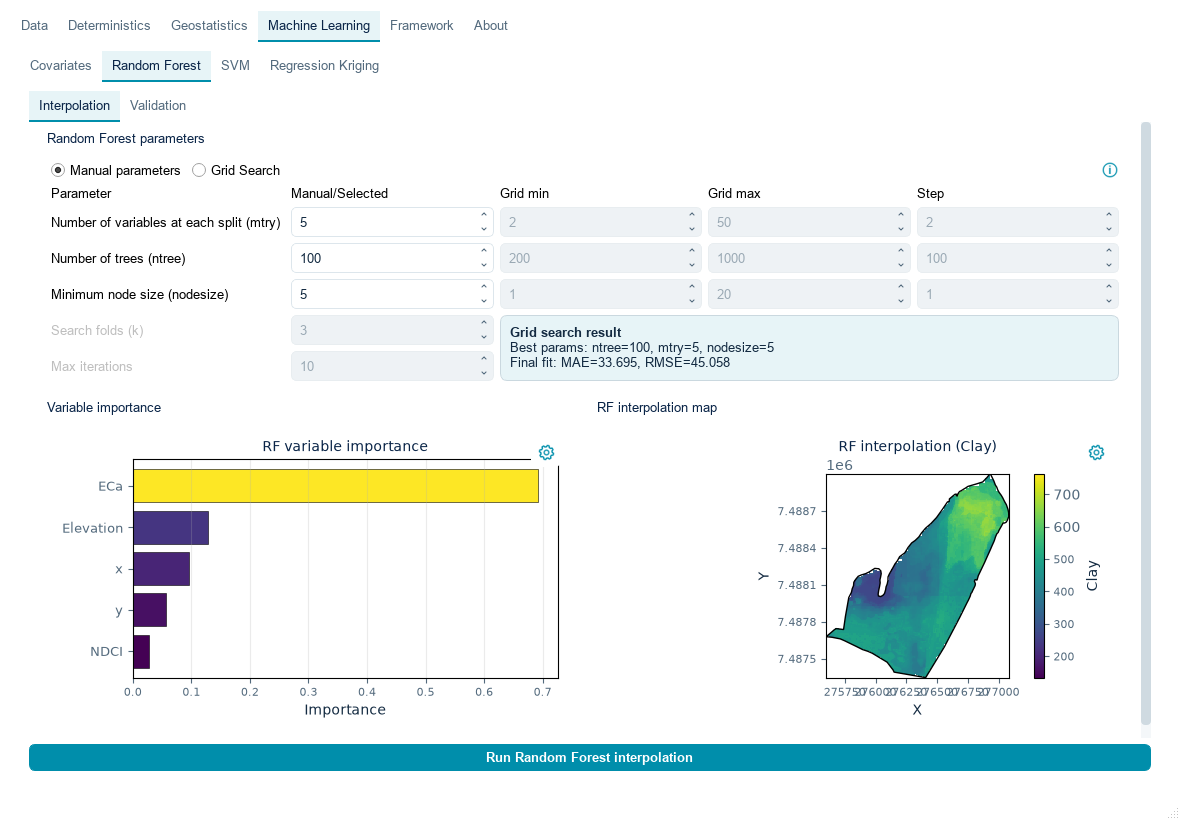
\includegraphics[width=0.94\textwidth,height=0.68\textheight,keepaspectratio]{random_forest.png}
    \caption{Random Forest interpolation tab showing parameter controls, Grid Search settings, variable importance, and the interpolated RF map.}
    \label{fig:rf-interpolation}
\end{figure}


The \texttt{Random Forest} tab contains two parameter modes, shown in the upper panel of Figure~\ref{fig:rf-interpolation}:


\begin{enumerate}
    \item \textbf{Manual parameters.} The user directly defines \texttt{mtry}, \texttt{ntree}, and \texttt{nodesize}. In this mode, the plugin fits the RF model once using the selected predictors and the parameter values entered by the user.


    \item \textbf{Grid Search.} The user defines a search range for each RF parameter using \texttt{Grid min}, \texttt{Grid max}, and \texttt{Step}. The plugin builds candidate values from those ranges and evaluates parameter combinations until the \texttt{Max iterations} limit is reached. The \texttt{Search folds (k)} value controls how many cross-validation folds are used internally to compare candidate parameter sets during the search. Grid Search is therefore used to find suitable RF hyperparameters for the selected predictor set; it does not select covariates by itself.
\end{enumerate}


The RF parameters in Figure~\ref{fig:rf-interpolation} control different parts of the model:


\begin{itemize}
    \item \texttt{mtry}: number of predictor variables randomly considered at each split in each tree. If many predictors are selected, a smaller \texttt{mtry} makes the trees more different from each other; a larger \texttt{mtry} lets each split evaluate more variables and may favor dominant predictors.


    \item \texttt{ntree}: number of trees grown in the forest. Increasing \texttt{ntree} usually makes the prediction more stable because the final map averages more trees, but it also increases processing time and memory use.


    \item \texttt{nodesize}: minimum number of samples allowed in a terminal node. Smaller values allow trees to follow finer local patterns in the training data; larger values make each tree smoother and more generalized.
\end{itemize}


In Grid Search, the \texttt{Step} value determines how the candidate list is created between the minimum and maximum values. A small step explores the range more finely but creates more candidate combinations, while a larger step reduces processing time by testing fewer values. The same logic applies separately to \texttt{mtry}, \texttt{ntree}, and \texttt{nodesize}.


After the model is fitted, the lower panels of Figure~\ref{fig:rf-interpolation} display the RF interpolation map and the variable-importance plot. The importance plot helps identify which selected predictors contributed most to the RF model. This result should be interpreted together with the covariate correlation matrix because a variable can appear important while still being redundant with another predictor.


\begin{infobox}
RF results depend on the quality and relevance of the selected predictors. Including \texttt{x} and \texttt{y} can help the model represent broad spatial trends, but the final predictor set should still be checked carefully. Weak, redundant, poorly aligned, or incomplete covariates can reduce model performance even when the interpolation runs successfully.
\end{infobox}


\subsubsection{Support Vector Machine}


Support Vector Machine (SVM) is also implemented as a spatial machine learning interpolation method in the plugin. As with RF, the model can use the point coordinates, \texttt{x} and \texttt{y}, together with the raster covariates prepared in the \texttt{Covariates} tab. The selected predictors are used to train the model and to generate predictions over the interpolation grid.


Before running SVM, complete the covariate preparation workflow and select the final predictors when the plugin asks which variables should be used. The selected set may include only raster covariates, only coordinates, or a combination of \texttt{x}, \texttt{y}, and raster covariates, depending on the interpolation objective and the available information.


Figure~\ref{fig:svm-interpolation} shows the SVM interpolation window. The left panel contains the manual and Grid Search controls, and the right panel shows the SVM interpolation map produced after fitting the model.


\begin{figure}[H]
    \centering
    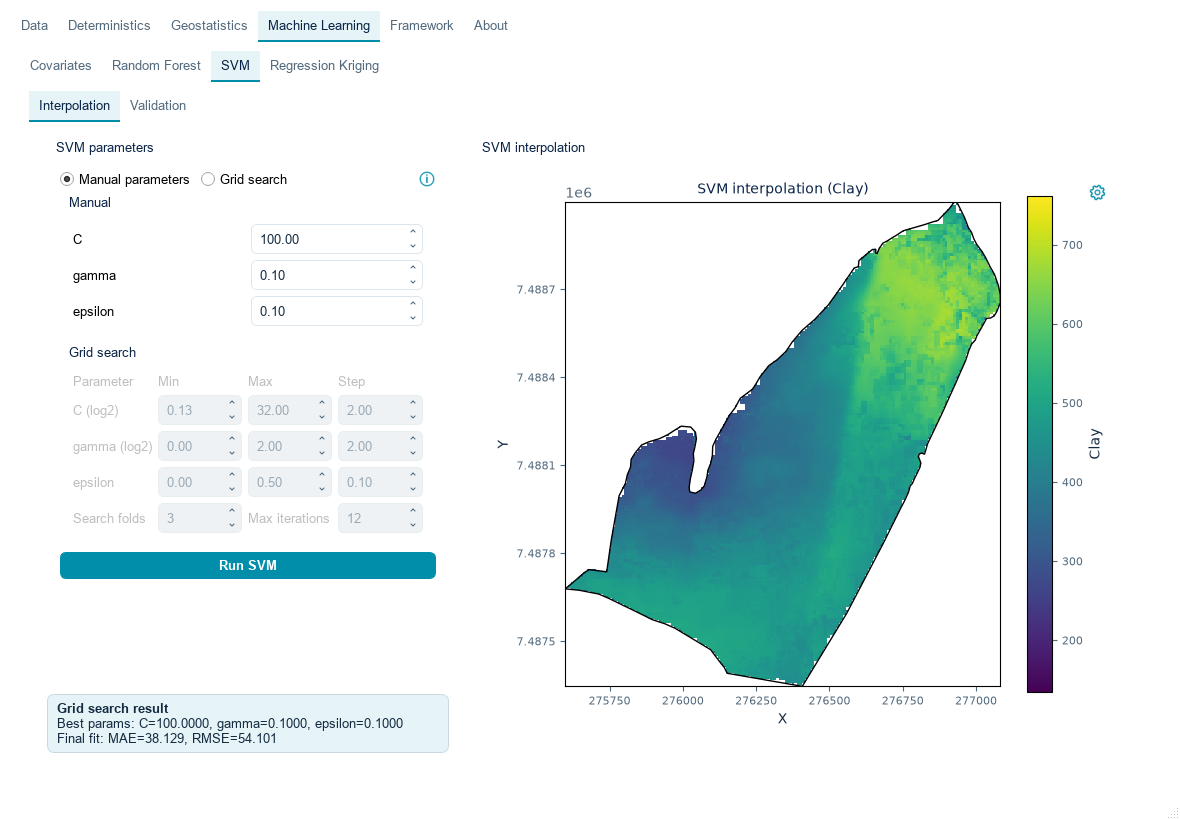
\includegraphics[width=0.94\textwidth,height=0.68\textheight,keepaspectratio]{svm.png}
    \caption{SVM interpolation on Paulínia with illustrative manual settings C=100, gamma=0.1, and epsilon=0.1. Validate or tune these settings for the mapping objective.}
    \label{fig:svm-interpolation}
\end{figure}


The \texttt{SVM} tab contains two parameter modes, shown in the left panel of Figure~\ref{fig:svm-interpolation}:


\begin{enumerate}
    \item \textbf{Manual parameters.} The user directly defines \texttt{C}, \texttt{gamma}, and \texttt{epsilon}. In this mode, the plugin fits the SVM model once using the selected predictors and the parameter values entered by the user.


    \item \textbf{Grid Search.} The user defines minimum, maximum, and step values for \texttt{C}, \texttt{gamma}, and \texttt{epsilon}. The plugin builds candidate parameter values and evaluates combinations until the \texttt{Max iterations} limit is reached. The \texttt{Search folds} value controls how many folds are used internally to compare candidate parameter sets during the search. Grid Search is used to tune SVM hyperparameters for the selected predictor set; it does not select covariates automatically.
\end{enumerate}


The SVM parameters in Figure~\ref{fig:svm-interpolation} control how flexible or smooth the fitted model will be:


\begin{itemize}
    \item \texttt{C}: penalty applied to prediction errors. Higher \texttt{C} values force the model to fit the training data more strictly, while lower values allow a smoother model with more tolerance to errors.


    \item \texttt{gamma}: controls how local the influence of each sample is in the radial basis function kernel. Higher \texttt{gamma} values create more local and complex responses; lower values produce smoother and broader spatial patterns.


    \item \texttt{epsilon}: defines the insensitive margin around the regression function. Errors smaller than \texttt{epsilon} are ignored during training. Smaller values fit the data more tightly, while larger values produce a smoother model.
\end{itemize}


In the Grid Search table, \texttt{C} and \texttt{gamma} are defined on a log2 scale, while \texttt{epsilon} is defined on its original scale. The \texttt{Step} value controls how many candidate values are created between the minimum and maximum settings. Smaller steps explore the search space more finely but increase processing time; larger steps reduce the number of combinations tested.


\begin{infobox}
SVM is sensitive to predictor scale. The current fitting pipeline standardizes the selected predictors internally. The Covariates tab also provides explicit \texttt{Z-score} and \texttt{Range [-1,1]} tools for preparing shared inputs; record any transformation used. Predictor scaling does not replace parameter tuning and independent validation.
\end{infobox}


\subsubsection{Regression Kriging}


Regression Kriging (RK) is implemented in the plugin as a hybrid interpolation method. It combines a Random Forest trend model with residual kriging. In the first stage, RF uses the selected predictors, such as \texttt{x}, \texttt{y}, and raster covariates, to model the deterministic or explanatory component of the target variable. In the second stage, the residuals from the RF model are interpolated with kriging to account for spatial structure that remains after the covariate-based prediction.


Before running RK, complete the \texttt{Covariates} workflow and select the final predictors when the plugin requests them. Because the RF stage is the base of RK, the predictor-selection logic is the same as in the RF tab: only the selected variables are used to fit the trend, estimate residuals, tune RF parameters, and build the final map.


Figure~\ref{fig:rk-interpolation} shows one Regression Kriging workspace with the RF trend and residual kriging panels side by side. The diagnostic area includes the residual semivariogram and variable importance, beside the RK map. The fitting controls belong to Interpolation; Validation is used to assess the configured RK result.


\begin{figure}[H]
    \centering
    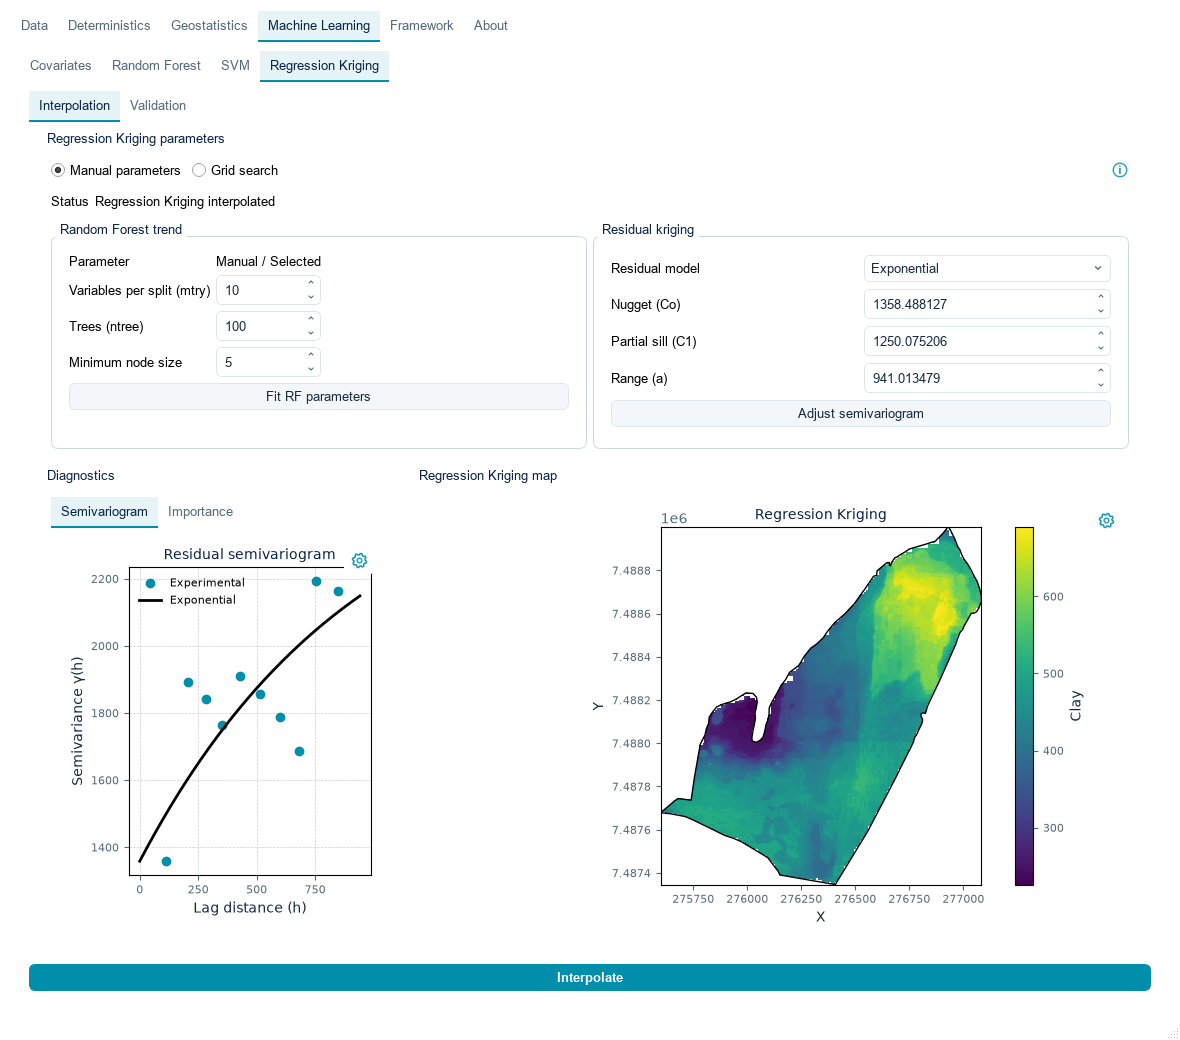
\includegraphics[width=0.94\textwidth,height=0.68\textheight,keepaspectratio]{regression_kriging.png}
    \caption{Regression Kriging tab showing the Random Forest trend settings, residual kriging parameters, residual semivariogram, and final RK interpolation map.}
    \label{fig:rk-interpolation}
\end{figure}


The RK workflow has two main parameter groups:


\begin{enumerate}
    \item \textbf{Random Forest trend.} The RF component uses \texttt{mtry}, \texttt{ntree}, and \texttt{nodesize}, with the same interpretation described for the RF method. These parameters can be entered manually or searched using \texttt{Grid search}. The \texttt{Fit RF parameters} button fits or tunes the RF trend and reports the selected RF parameter combination.


    \item \textbf{Residual kriging.} After the RF trend is fitted, the plugin models the residuals using a residual variogram. The user can choose the residual variogram model and review or adjust the kriging parameters before clicking \texttt{Interpolate}.
\end{enumerate}


The residual kriging controls in Figure~\ref{fig:rk-interpolation} describe the spatial dependence left in the RF residuals:


\begin{itemize}
    \item \texttt{Residual variogram model}: theoretical model fitted to the residual semivariogram. The interface provides \texttt{Spherical}, \texttt{Exponential}, and \texttt{Gaussian} options.


    \item \texttt{Nugget (Co)}: residual semivariance at very short distances, including measurement error or micro-scale variation not captured by the RF trend.


    \item \texttt{Partial sill (C1)}: structured residual variance explained by spatial dependence.


    \item \texttt{Range (a)}: distance at which residual spatial correlation becomes weak or negligible.
\end{itemize}


The residual semivariogram panel helps verify whether the RF residuals still show spatial dependence. If the residuals have a meaningful spatial pattern, RK can improve the final map by adding a kriged residual surface to the RF trend prediction. If the residual structure is weak, the RK map may be very similar to the RF map.


\begin{infobox}
RK should be interpreted as a hybrid method rather than a purely machine learning method. The RF stage explains variation using coordinates and covariates, while the kriging stage models spatial autocorrelation remaining in the residuals. Its performance therefore depends on both predictor quality and the quality of the residual variogram.
\end{infobox}



\subsubsection{Adjusting the Residual Semivariogram}

After fitting the RF trend with \texttt{Fit RF parameters}, click \texttt{Adjust semivariogram} in the residual panel. The popup exposes maximum distance, lag distance or number of lags, and the candidate models without separating the RF and kriging workspace into two windows.

Click \texttt{Update preview} after changing distance or lag settings. Click \texttt{Validate models} to compare the selected Spherical, Exponential, and Gaussian candidates. In this residual adjustment workflow the selection uses the lowest RMSE, with SSE used to resolve a tie. Inspect the numerical table and select a row before \texttt{Apply selected model}. The rule is displayed in the window; Geostatistics prioritizes LCCC, while the Framework semivariogram popup prioritizes $R^2$.


\begin{figure}[H]
    \centering
    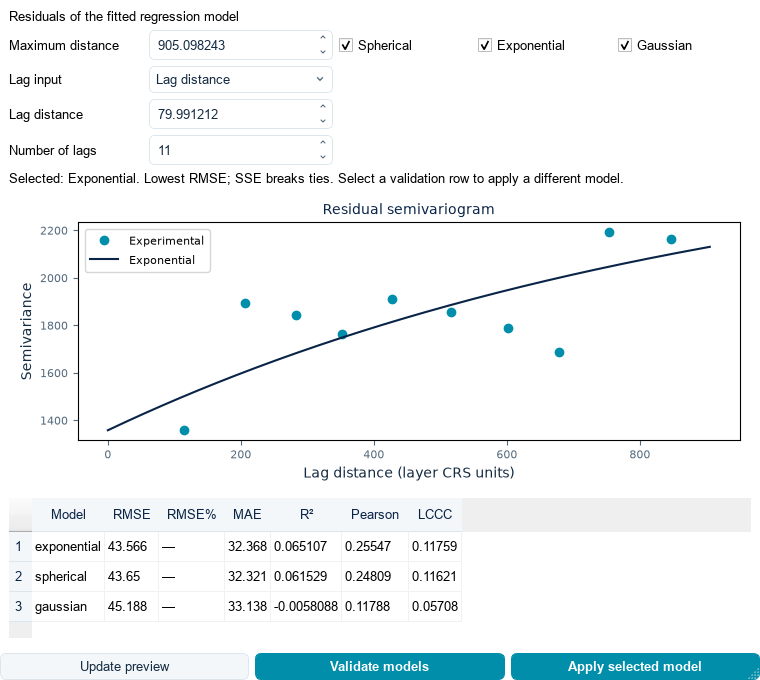
\includegraphics[width=0.85\textwidth,height=0.55\textheight,keepaspectratio]{residual_adjust.png}
    \caption{Residual semivariogram adjustment: distance and lag controls, model preview, numerical validation, and Apply selected model.}
    \label{fig:residual-adjust}
\end{figure}

Return to the RK workspace and click \texttt{Interpolate} to generate the sum of the RF trend and kriged residual prediction. Run RK validation from its \texttt{Validation} subtab. After changing the predictors, RF fit, or residual settings, recalculate the dependent stages rather than accepting an earlier result.


\section{Validation of the Selected Interpolator}


Validation is used to evaluate the result produced by the interpolator selected by the user. In the plugin, the validation tabs follow the same general structure across deterministic, geostatistical, and machine learning methods, but each validation result refers to the method currently being evaluated. The user can run validation from the corresponding method tab after the common inputs and method-specific parameters have been defined.


Figure~\ref{fig:validation-cross-validation} shows the common validation layout. The observed-versus-predicted plot displays the validation points, the 1:1 reference line, and the fitted trend line. The metrics panel reports the numerical validation results, while the controls below it allow the user to choose between automatic CV, LOOCV, and K-Fold.


\begin{figure}[H]
    \centering
    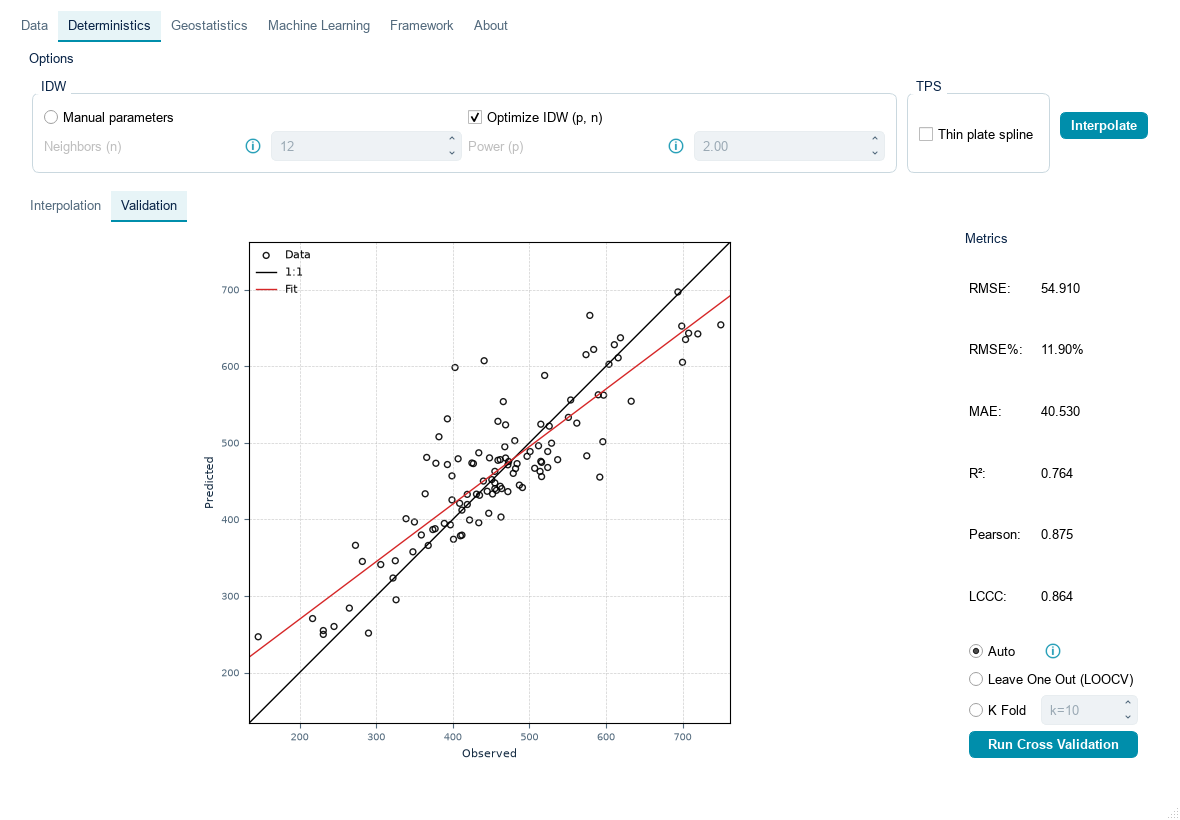
\includegraphics[width=0.94\textwidth,height=0.68\textheight,keepaspectratio]{validation.png}
    \caption{Validation tab showing the observed-versus-predicted plot, validation metrics, and cross-validation mode controls.}
    \label{fig:validation-cross-validation}
\end{figure}


The available validation modes are:


\begin{enumerate}
    \item \textbf{Auto.} The plugin selects the validation strategy according to the number of valid observations used by the method. If the dataset has \(n \leq 100\) valid observations, the plugin uses Leave-One-Out Cross-Validation (LOOCV). If the dataset has \(101 \leq n \leq 500\), the plugin uses K-Fold cross-validation with \(k = 10\). If the dataset has more than 500 valid observations, the plugin uses K-Fold cross-validation with \(k = 5\). This is the general automatic CV rule. Massive-data validation uses the disclosed bounded hold-out workflow described in Section~\ref{sec:dense-validation}.


    \item \textbf{Leave-One-Out Cross-Validation (LOOCV).} The plugin removes one observation at a time, fits or predicts using the remaining observations, and validates the prediction at the omitted location. LOOCV uses all possible single-point omissions and is useful for small datasets, but it can be slow when the number of observations is large.


    \item \textbf{K-Fold Cross-Validation.} The plugin randomly divides the observations into \(k\) groups. For each fold, one group is used for validation and the remaining groups are used for fitting or prediction. K-Fold is faster than LOOCV for medium and large datasets because it requires fewer validation runs.
\end{enumerate}


The value of \(n\) refers to the valid observations available to the method at validation time. For machine learning methods, this means observations with the target variable and complete values for the selected predictors. If missing covariate values are present, the number of valid observations used for validation may be smaller than the original point-layer count.


Validation outputs are reported through metrics and observed-versus-predicted plots, as illustrated in Figure~\ref{fig:validation-cross-validation}. The metrics evaluate the selected interpolation run and may include RMSE, RMSE\%, MAE, $R^2$, Pearson correlation, and LCCC, depending on the method tab. Lower error metrics indicate smaller prediction errors, while higher agreement or correlation metrics indicate stronger agreement between observed and predicted values.


\begin{infobox}
Validation evaluates how the selected interpolator predicts values at sampled locations, not how visually smooth or detailed the output map appears. A visually detailed map is not necessarily more reliable, so the validation metrics and observed-versus-predicted plot should be checked before accepting the interpolation result.
\end{infobox}


\section{Framework-Guided Interpolation}

The Framework tab is not an additional interpolation model. It is a decision-support component that organizes the information already loaded in the plugin and guides the choice of an interpolation route. This framework is based on the scientific criteria described by \cite{delgadobejarano2026}, so the recommendation is not arbitrary; it follows data characteristics and spatial evidence. The plugin uses two possible framework paths, depending on whether auxiliary covariate rasters are available.

\subsection{Framework Overview and Data}

The first window in the Framework tab is an overview of the current dataset. This screen brings together the information needed before choosing the framework path. The target variable, pixel size, and number of samples come from the selections made in the Data tab. Moran's I, the p-value, the spatial pattern, the Spatial Dependence Index (SDI), and the SDI status summarize the spatial diagnosis used by the framework. The semivariogram preview is calculated automatically from the current data using the active Geostatistics semivariogram configuration. It is synchronized as soon as the Framework preview is displayed, and the same configuration can be edited through \textit{Semivariogram settings}.

\begin{figure}[H]
    \centering
    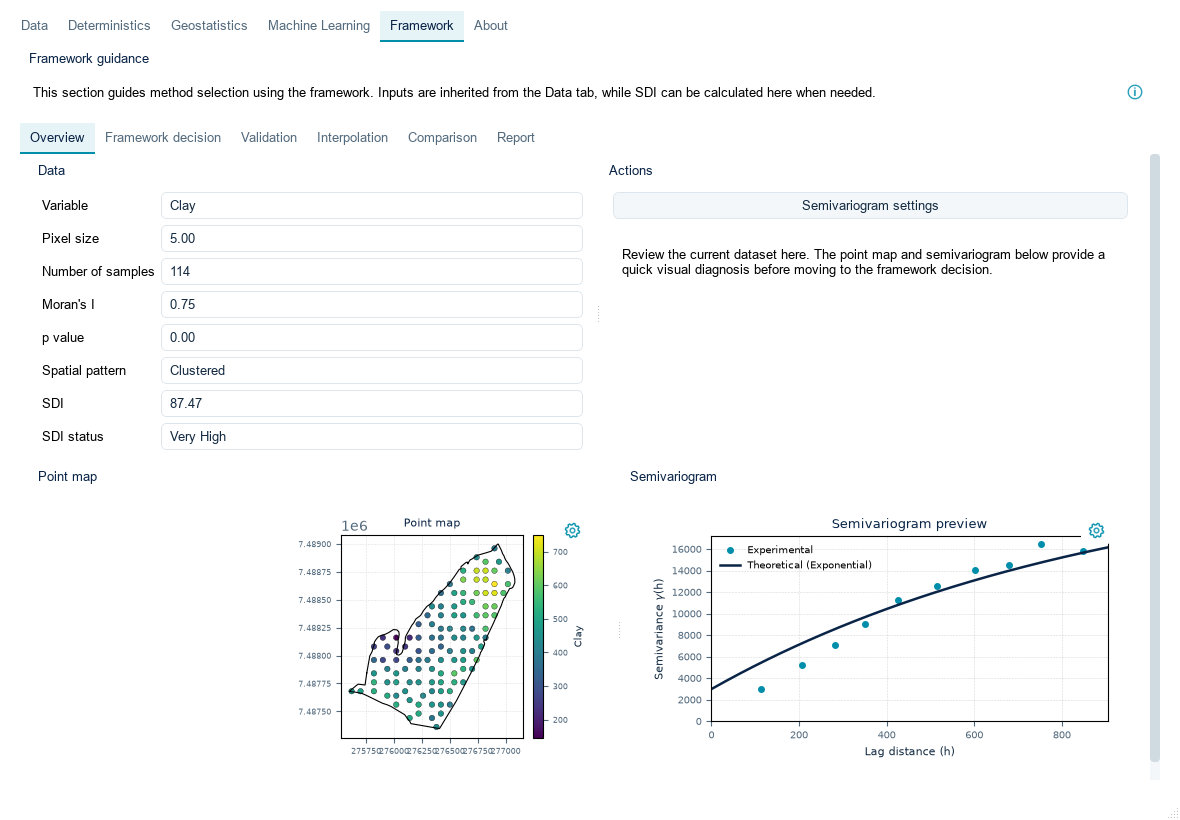
\includegraphics[width=0.95\textwidth]{framework_overview.png}
    \caption{Framework overview showing the dataset information, point map, and semivariogram preview used before choosing the framework path.}
    \label{fig:framework-overview-data}
\end{figure}

The point map and semivariogram preview provide a visual check before moving to the \textit{Framework decision} tab. The point map helps verify the sampled values and their distribution within the boundary polygon. The semivariogram preview helps the user identify whether there is spatial structure that may justify a geostatistical route. If the automatic semivariogram does not represent the dataset adequately, the user can adjust the model settings before continuing. At this stage, the user is reviewing the dataset and the spatial evidence that will support the framework decision.

\subsection{Framework Decision Paths}

After the overview has been checked, the user selects the framework mode in the \textit{Framework decision} tab, as shown in Figure~\ref{fig:framework-decision-univariate}. The plugin provides two decision paths:

\begin{itemize}
    \item \textbf{Univariate framework}: used when the interpolation is based only on the sampled point layer, the target variable, the boundary polygon, the pixel size, and the spatial diagnostics. Covariate rasters are not used in this route. The available methods are TPS, OK, and IDW.
    \item \textbf{Full framework}: used when auxiliary raster covariates are available. When this mode is selected, the \textit{View covariates} option opens the same covariate-preparation window mentioned in \hyperref[sec:ml-covariates]{\textcolor{mainblue}{Section~\ref*{sec:ml-covariates}}} and shown in Figure~\ref{fig:ml-covariates}. The available methods are TPS, OK, IDW, SVM, RF, and RK.
\end{itemize}

The framework figure is dynamic. It is updated according to the characteristics of the current dataset, including sample size, spatial pattern, Moran's I significance, SDI, and the selected framework mode. After the user clicks \textit{Evaluate available methods}, the plugin follows the selected framework path and displays the suggested method in the decision summary and suggested-methods panel.

\begin{figure}[H]
    \centering
    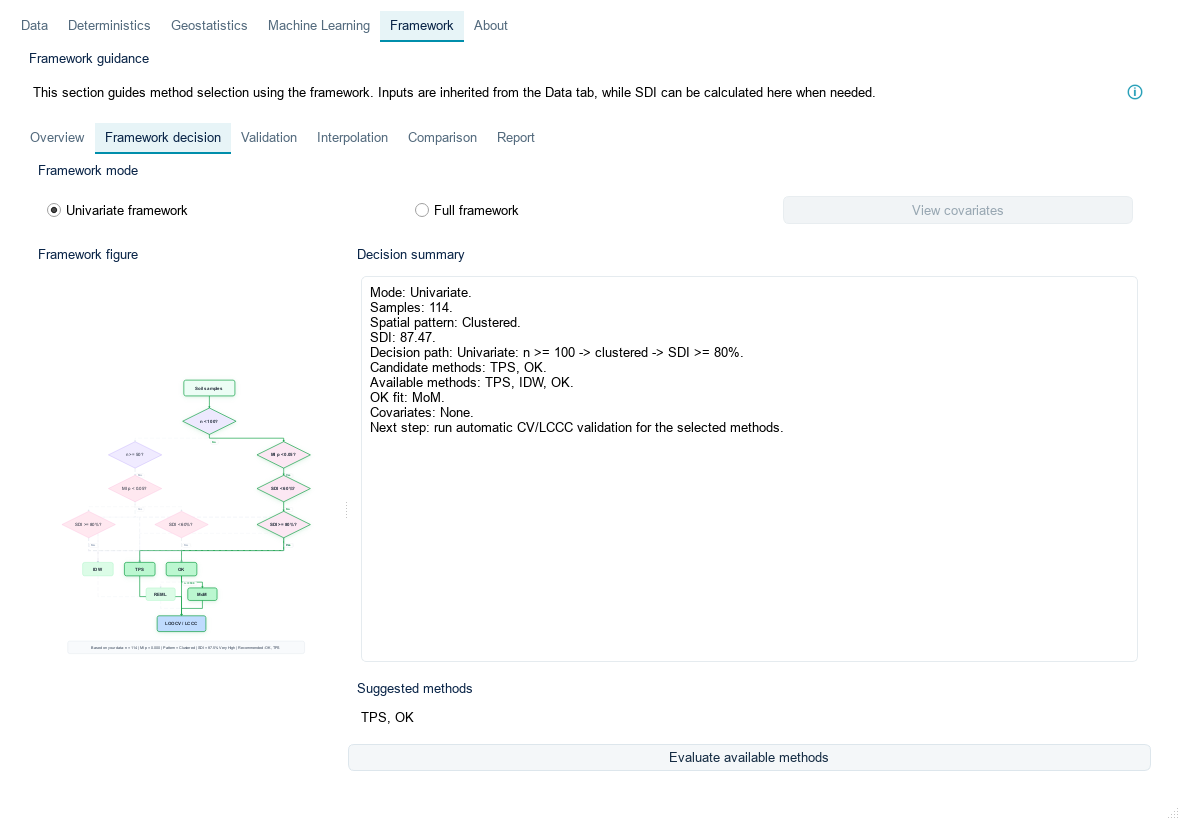
\includegraphics[width=0.95\textwidth]{framework_decision.png}
    \caption{Framework decision tab showing the framework mode selection, the univariate decision summary, and the suggested method for the current dataset.}
    \label{fig:framework-decision-univariate}
\end{figure}

\begin{infobox}
The overview screen is common to the framework workflow. It helps the user review the data, Moran's I, SDI, point distribution, and semivariogram before deciding whether the recommendation will follow the univariate route or the full framework with covariates.
\end{infobox}

\subsection{Framework Validation}

The Validation tab evaluates the methods selected within the framework workflow. After the framework decision has been generated, the plugin can automatically select the recommended methods through \textit{Select suggested}. The user can also manually activate additional methods before running validation. This is useful because the framework recommendation is a technical guide based on general data characteristics, not an absolute rule. For a given set of plugin settings, interpolation performance is strongly data-dependent and is affected by the structure, distribution, variability, and quality of the current dataset. Therefore, the framework should be interpreted as a decision-support tool that narrows the set of reasonable methods, while validation provides the empirical evidence for the selected data.

When the user clicks \textit{Run validation}, the plugin validates the selected methods and reports the results in a table. The table includes error, agreement, and correlation metrics such as RMSE, RMSE\%, MAE, $R^2$, Pearson correlation, and LCCC. The validation summary identifies the winner among the methods included in that validation run. The Framework ranks methods by the highest LCCC and then the lowest RMSE; this method ranking differs from the semivariogram model ranking.

\begin{figure}[H]
    \centering
    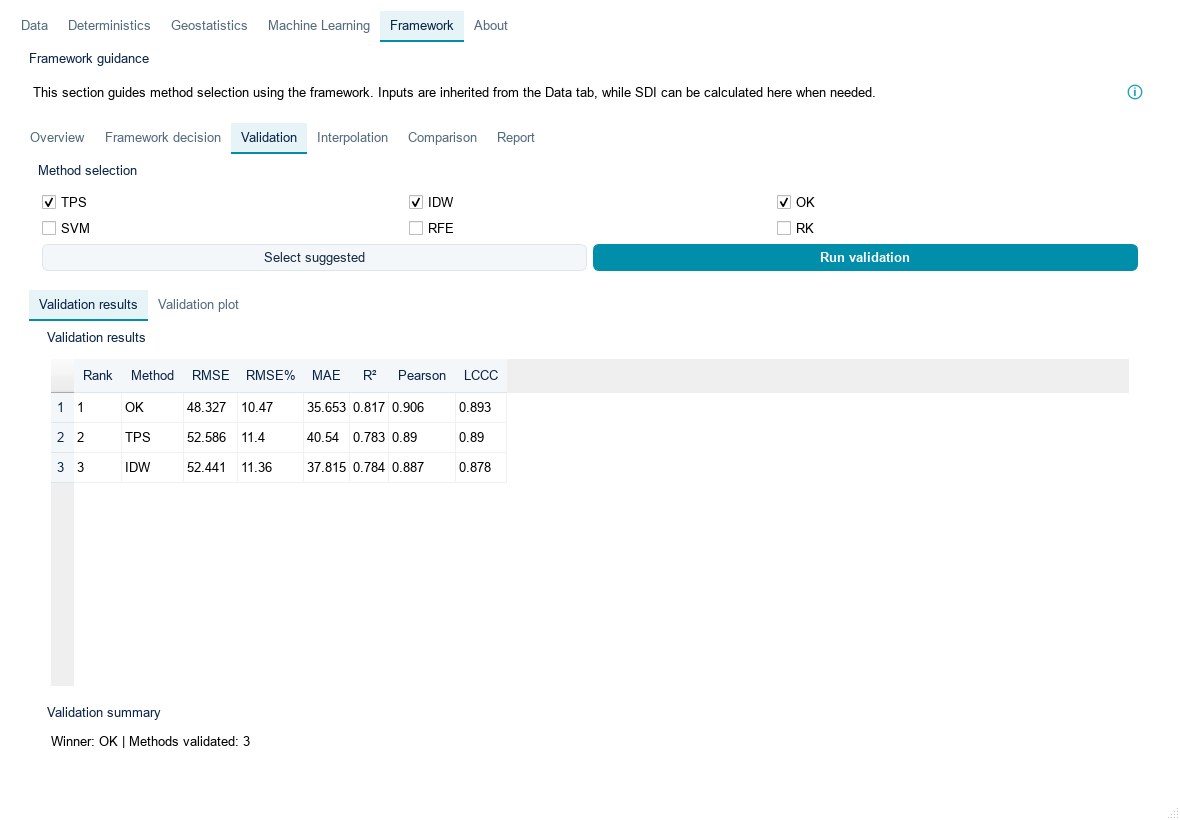
\includegraphics[width=0.95\textwidth]{framework_validation.png}
    \caption{Framework validation tab showing method selection, the validation results table, and the validation summary for the selected methods.}
    \label{fig:framework-validation-results}
\end{figure}

The Validation plot tab provides graphical support for interpreting the results. The user can compare the selected methods through LCCC and RMSE plots. Higher LCCC indicates stronger agreement between observed and predicted values, while lower RMSE indicates smaller prediction error. In addition, the user can inspect observed-versus-predicted plots for each selected method, which helps identify bias, dispersion, or systematic under- and over-prediction.

\begin{figure}[H]
    \centering
    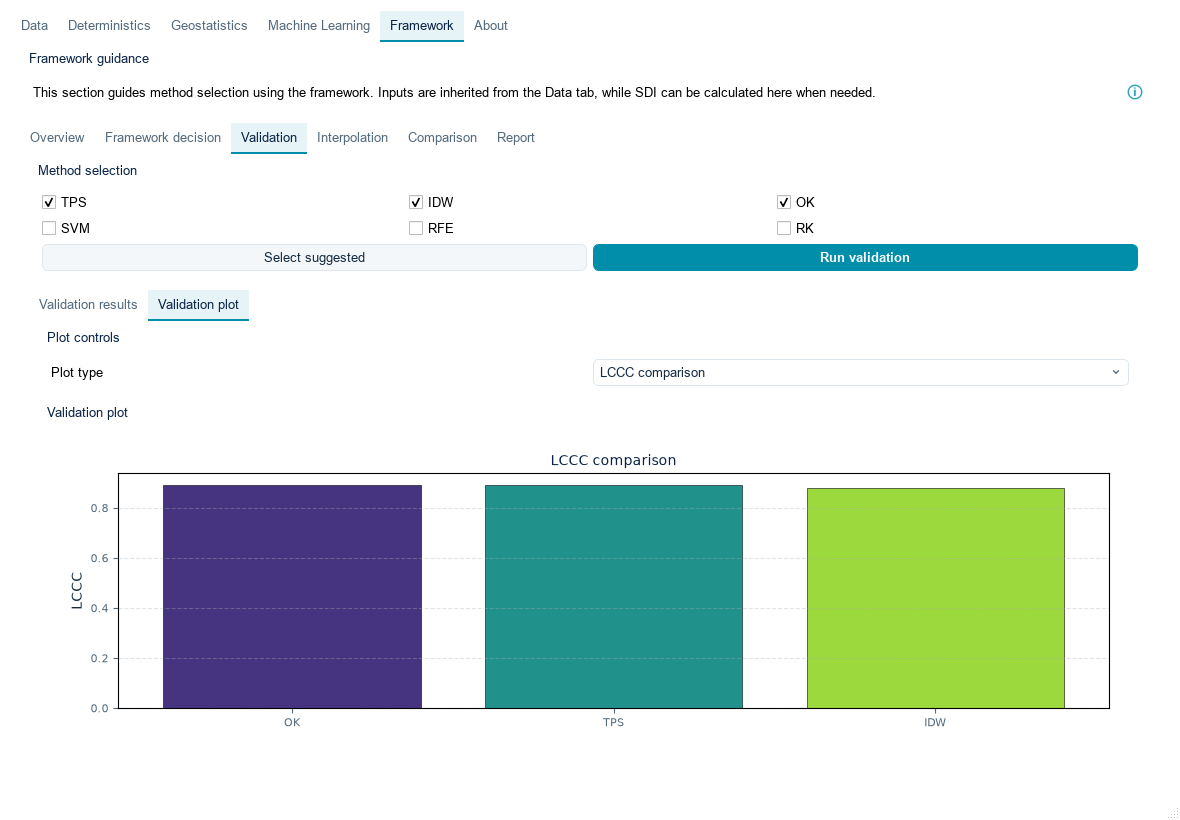
\includegraphics[width=0.95\textwidth]{framework_validation_plot.png}
    \caption{Framework validation plot tab showing graphical comparison of the selected methods using LCCC; RMSE comparison and observed-versus-predicted plots can also be selected.}
    \label{fig:framework-validation-plot}
\end{figure}

\begin{infobox}
The method suggested by the framework is the method expected to be suitable according to the framework criteria, but the final decision should also consider the validation metrics and plots obtained for the current dataset.
\end{infobox}

\subsection{Final Decision and Interpolation}

The \texttt{Interpolation} page uses the best validated method by default while \texttt{Use best validated method} is active. Disable this option to select another available validated method. Changing the selection prepares the next run; it does not change a raster already generated.

Click \texttt{Run interpolation} to generate the final Framework map. The summary distinguishes the framework recommendation, validation winner, selection for the next run, and the method actually interpolated. The Report describes the executed interpolation. For example, choosing IDW after running TPS leaves the report's executed method as TPS until a new IDW interpolation finishes successfully.


\begin{figure}[H]
    \centering
    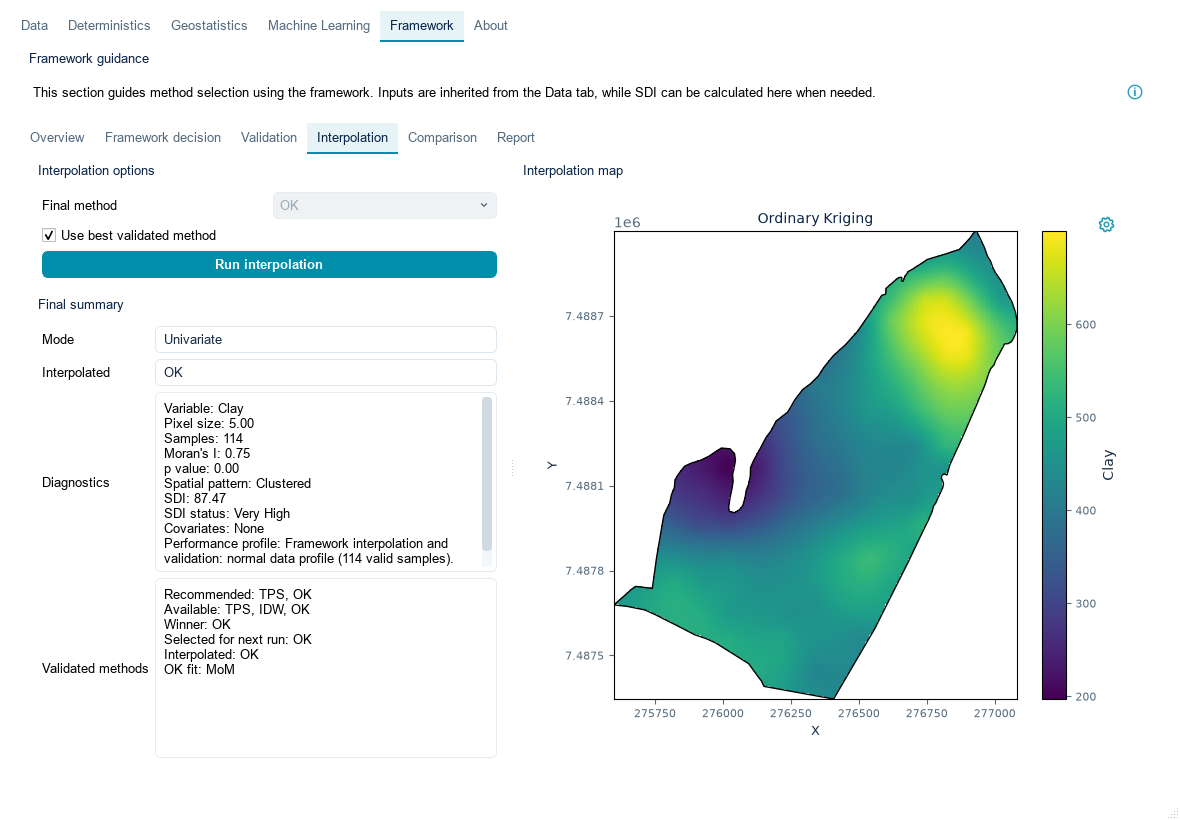
\includegraphics[width=0.97\textwidth,height=0.60\textheight,keepaspectratio]{framework_interpolation.png}
    \caption{Framework interpolation page: final method selection, map, and executed-result summary.}
    \label{fig:framework-final-report}
\end{figure}

\subsection{Validating Models in Framework Semivariogram Settings}

From \texttt{Overview}, click \texttt{Semivariogram settings}. Review the fitting method, maximum distance, lag distance or lag count, model, nugget, partial sill, and range. \texttt{MoM} shows experimental semivariances and a theoretical curve; \texttt{REML} shows the theoretical curve only.


\begin{figure}[H]
    \centering
    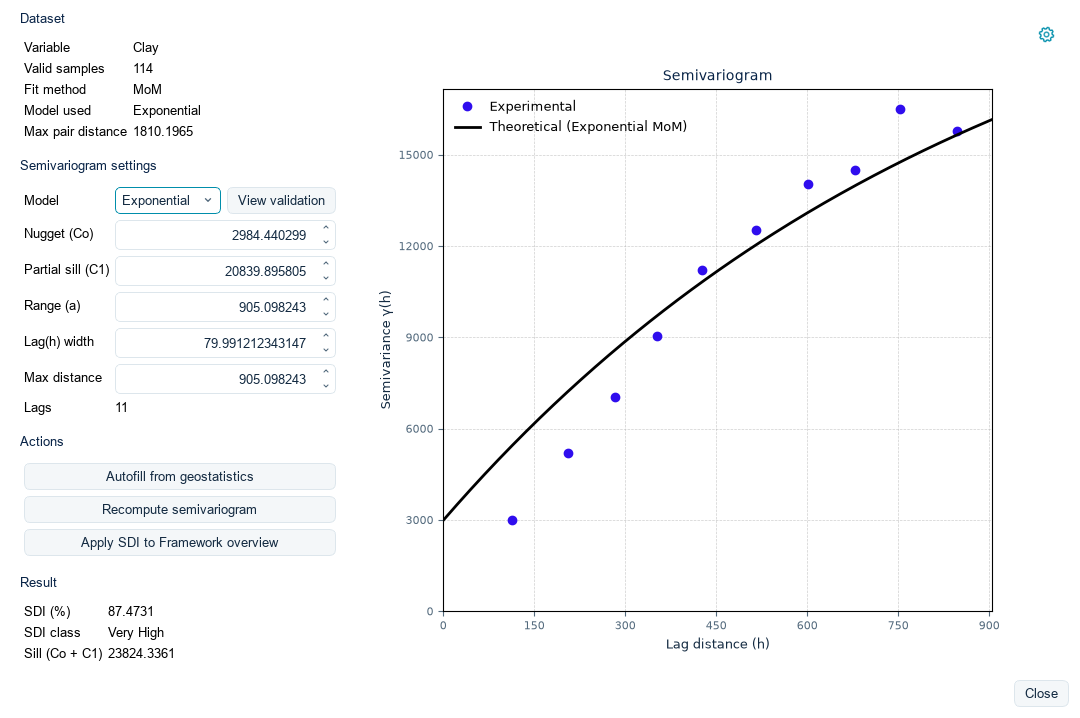
\includegraphics[width=0.97\textwidth,height=0.52\textheight,keepaspectratio]{framework_semivariogram_settings.png}
    \caption{Framework semivariogram settings with model validation beside the current distance, lag, and parameter controls.}
    \label{fig:framework-semivariogram-settings}
\end{figure}

Click \texttt{View validation} to compare Spherical, Exponential, and Gaussian models with the current data and settings. The table reports cross-validation metrics and explains the automatically recommended model: highest $R^2$, then lowest RMSE. Select a successful candidate row and click \texttt{Apply selected model} to use its fitted parameters. Review the new SDI and apply it to the Framework overview when appropriate.


\begin{figure}[H]
    \centering
    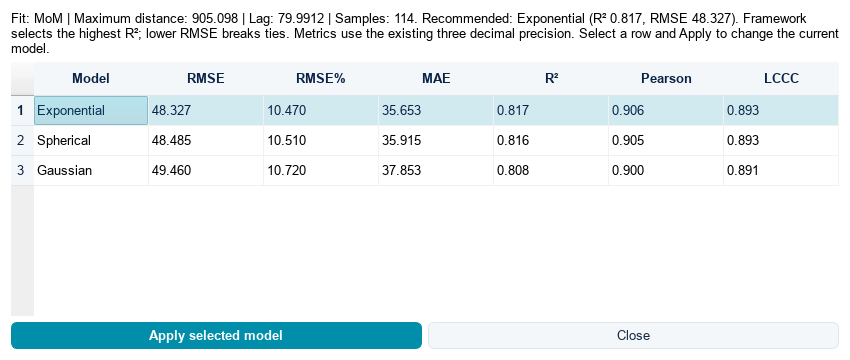
\includegraphics[width=0.97\textwidth,height=0.37\textheight,keepaspectratio]{framework_model_validation.png}
    \caption{Framework model validation: all three candidates, ranking explanation, and Apply selected model.}
    \label{fig:framework-model-validation}
\end{figure}

If the data or settings change while validating, reopen validation for the current configuration. An earlier table should not be used to apply stale parameters.

\section{Comparison of Maps}
\label{sec:map-comparison}

The Framework \texttt{Comparison} page compares maps. Quantitative method-validation results remain in \texttt{Validation}. Use both views: validation assesses prediction error, whereas map comparison shows where spatial predictions differ.

\begin{enumerate}
    \item Validate the candidate methods using the current input data. In Full mode, prepare covariates before validating RF, SVM, or RK.
    \item Open \texttt{Comparison}. Choose two different available methods in \texttt{Map A} and \texttt{Map B}. Validated alternatives are listed even if their maps have not yet been generated.
    \item Click \texttt{Compare maps}. The plugin generates missing candidate maps on the current grid, then displays A, B, and their signed difference. Comparison does not replace the executed final Framework result.
    \item Read the difference as $D=A-B$. Positive cells mean A predicts a higher value; negative cells mean B predicts a higher value. The difference uses the target variable's units. Reversing A and B reverses the sign.
    \item Click the corner configuration button to use a common palette, value range, and extent. Compare A and B with a shared value range so that equal colors represent equal values. The difference has its own diverging color scale.
    \item Pan or zoom to inspect the same area in both maps. Use \texttt{Fit to layer} to return to the full extent.
    \item Enable \texttt{Include this comparison in report} after producing the comparison you want to document.
\end{enumerate}


\begin{figure}[H]
    \centering
    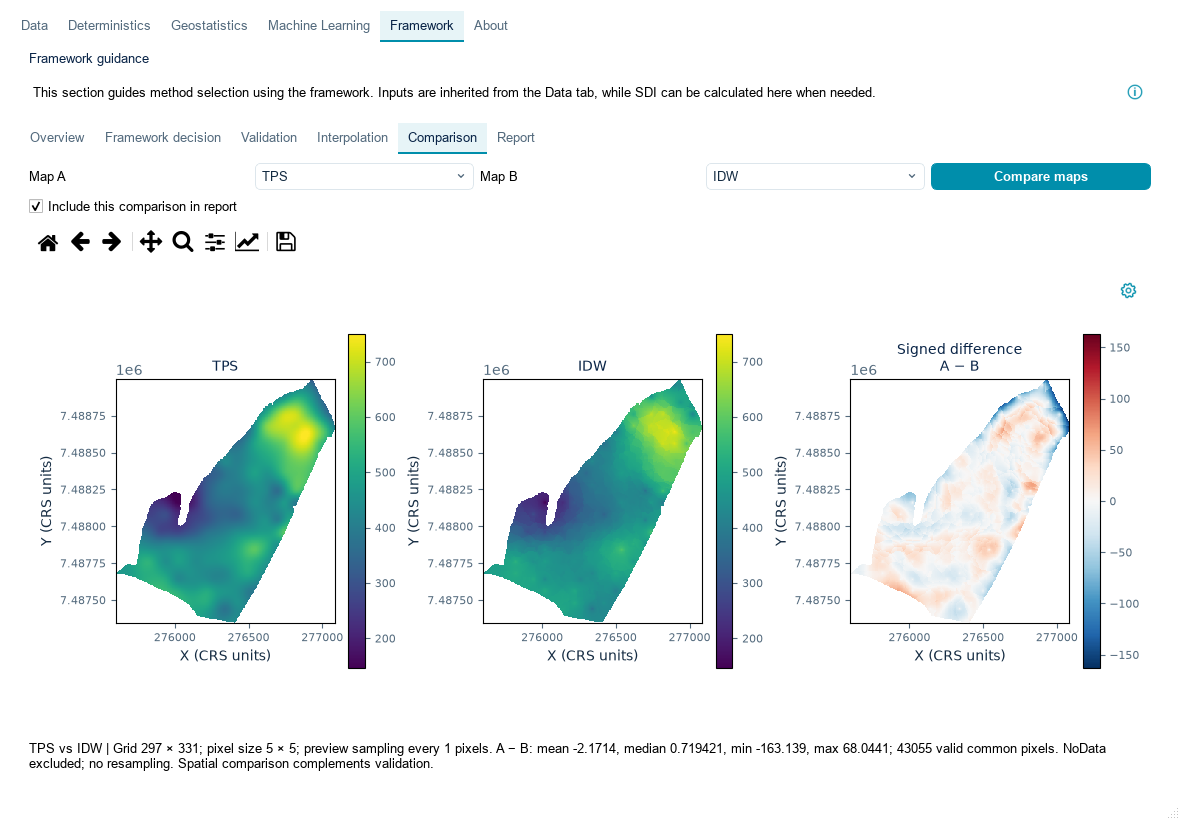
\includegraphics[width=0.97\textwidth,height=0.60\textheight,keepaspectratio]{map_comparison.png}
    \caption{Comparison page with Map A, Map B, and the signed A minus B map on the common raster grid.}
    \label{fig:map-comparison}
\end{figure}

The rasters must have the same CRS, grid dimensions, geotransform, pixel size, and alignment. The calculation excludes pixels with NoData in either map and does not resample incompatible grids. Difference statistics use all valid common pixels; large-grid previews may display a sampled rendering, which is disclosed in the status line. A small mean difference can hide large positive and negative local differences, so inspect the map, range, and distribution as well.

If a candidate map cannot be generated, inspect the status message and correct its prerequisites, such as missing predictors or a failed model. The previously executed final map remains recorded. Changing the candidate selection invalidates the earlier comparison and requires \texttt{Compare maps} again.

\section{Map Display and Larger View}

Spatial maps have a configuration button in the plot corner. It opens a popup with visible color gradients, palette selection, automatic or manual value limits, numeric scale, and \texttt{Fit to layer}. These controls change the display, not the predictions or validation metrics. Numeric map scale requires a projected CRS and uses its map units.


\begin{figure}[H]
    \centering
    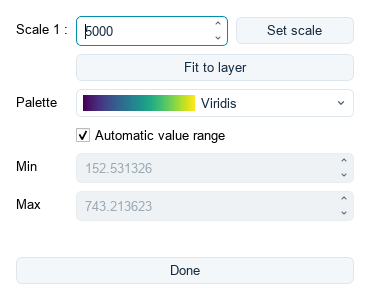
\includegraphics[width=0.65\textwidth,height=0.37\textheight,keepaspectratio]{map_settings.png}
    \caption{Map display settings: scale, fit, visible palette preview, and value range.}
    \label{fig:map-settings}
\end{figure}

\begin{figure}[H]
    \centering
    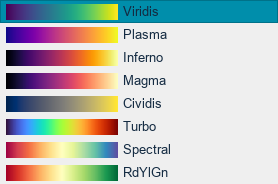
\includegraphics[width=0.57\textwidth,height=0.27\textheight,keepaspectratio]{palettes.png}
    \caption{The palette selector shows color gradients as well as palette names.}
    \label{fig:palettes}
\end{figure}


\begin{figure}[H]
    \centering
    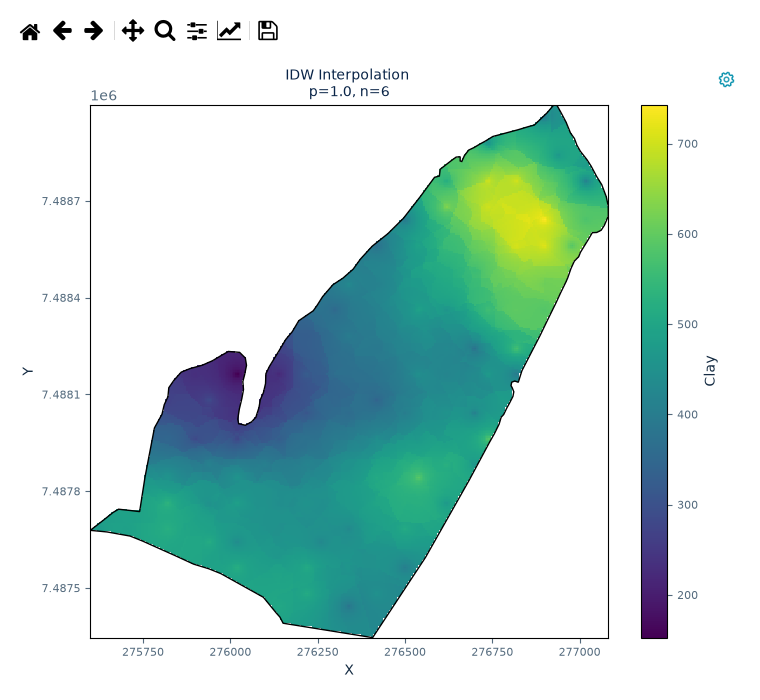
\includegraphics[width=0.83\textwidth,height=0.50\textheight,keepaspectratio]{larger_view.png}
    \caption{Enlarged map view retaining the current styling and its corner configuration button.}
    \label{fig:larger-view}
\end{figure}

Open \texttt{View larger view} from the plot context menu when a larger map is useful. The enlarged view preserves the map data, NoData mask, palette, value range, and current extent. Its corner configuration button opens the same display settings. Keep a common scale and color range when presenting comparable maps. Validation plots retain fixed scientific colors and do not offer a map-palette selector.

\section{Interactive Reports and Export}
\label{sec:reports}

The Framework \texttt{Report} page provides an interactive summary of the current session. Use the section list to review the overview, validation, interpolation, and diagnostics available for that session. The summary distinguishes a recommendation from the method actually executed and links back to the relevant analysis pages.


\begin{figure}[H]
    \centering
    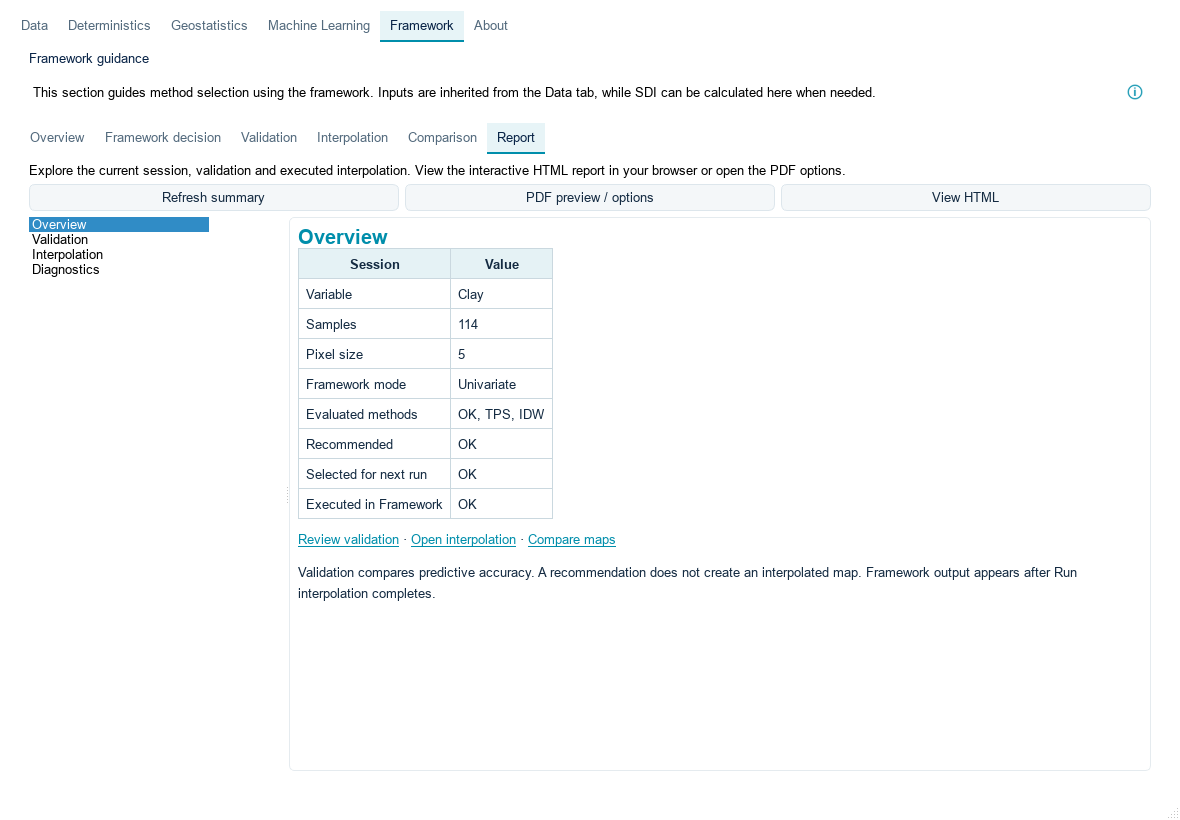
\includegraphics[width=0.97\textwidth,height=0.60\textheight,keepaspectratio]{report.png}
    \caption{Report page: interactive session summary with PDF options and View HTML.}
    \label{fig:interactive-report}
\end{figure}

\subsection{Temporary HTML Preview}

Click \texttt{View HTML} to open a temporary HTML report in the browser. No destination filename is required and the user does not need to download the HTML first. The report embeds its figures, provides navigation links to its sections, and lets the user expand or collapse sections individually or with \texttt{Expand all} and \texttt{Collapse all}. This temporary preview is convenient for reviewing the results during the session; save or export the material if it must be kept permanently.

\subsection{PDF and Raster Outputs}

Click \texttt{PDF preview / options} to choose report content, inspect the paginated preview, and export a PDF. Available content depends on completed analyses and can include the point map, semivariogram, covariates, validation metrics and plots, framework decision, final interpolation, diagnostic results, and the included map comparison. A report can only document analyses that have actually been run.

Raster persistence is controlled by \texttt{Export Rasters to project folder} in \texttt{Data}. Enable it before interpolation to write the raster in the project output directory. If it is disabled, preserve a required temporary layer through QGIS export before closing the application. Keep the raster, report, parameter settings, data exclusions, and software environment together to document a mapping decision.

\section{Dense and Massive Datasets}
\label{sec:dense-massive}

The processing profile is selected automatically from the number of valid observations available to the current method. Density here names a computational profile based on sample count; it is not a physical sampling-density measurement. Missing values, missing predictors, and explicit exclusions may make this count smaller than the source layer's feature count.

\begin{table}[H]
\centering
\caption{Automatic processing profiles. Boundary counts belong to the lower profile.}
\label{tab:data-profiles}
\begin{tabularx}{0.96\textwidth}{P{2cm}P{3cm}Y}
\toprule
\textbf{Profile} & \textbf{Valid observations} & \textbf{Main implication} \\
\midrule
Normal & $n\leq500$ & Original small-sample processing paths \\
Dense & $500<n\leq10{,}000$ & Bounded tuning, local spatial prediction, and sampled variogram pairs \\
Massive & $n>10{,}000$ & Smaller prediction blocks and a bounded validation hold-out \\
\bottomrule
\end{tabularx}
\end{table}

There is no fixed stop at 100,000 observations. Productivity and sensor datasets around this scale and above can use the massive profile. Practical capacity depends on memory, output grid cells, covariates, neighborhood size, and the method. The 50,000-observation computational notice is advisory rather than a hard ceiling. A 32-bit QGIS process has a smaller address space than a 64-bit installation.

\subsection{What Changes with the Profile}

\begin{itemize}
    \item \textbf{Machine learning tuning.} Dense search limits the requested tuning to at most three folds and eight parameter candidates. Hyperparameter search uses a reproducible subset of at most 2,000 valid rows where needed. This search subset is separate from the final fit, which uses all valid rows available to that model.
    \item \textbf{Random Forest.} In massive mode, the resolved forest is bounded to at most 300 trees and a minimum terminal-node size of 5, including manually requested settings. Review the resolved parameters shown by the run.
    \item \textbf{SVM.} Above 500 observations, the scalable path uses an approximate kernel representation rather than the small-sample exact radial-basis SVR path. It uses up to 256 Nystroem components for dense data and 128 for massive data. Interpret this as a computational approximation and validate its suitability.
    \item \textbf{Ordinary and residual kriging.} Dense prediction uses local systems with a maximum neighborhood of 64 samples and a minimum of 16 where the available neighborhood permits. MoM replaces expensive REML fitting for large sample counts.
    \item \textbf{TPS.} Dense and massive profiles use local neighborhoods of 64 and 32 observations, respectively. This is a change from the global spline used with normal datasets.
    \item \textbf{Semivariogram.} Dense fitting bounds the sampled pair budget to 250,000 and proposes at most 36 lag classes; massive mode proposes at most 24. The displayed fit records the data profile. Pair sampling limits the calculation rather than deleting source observations.
    \item \textbf{Prediction and plotting.} Large predictions are processed in blocks; the shared block sizes are 25,000 rows for dense data and 5,000 for massive data where used. Point previews may use up to 10,000 representative samples; plots above 50,000 observations may use hexagonal density bins. A display sample does not define the final fitting population or raster statistics.
\end{itemize}

\subsection{Validation for Large Data}
\label{sec:dense-validation}

The general Auto rule uses LOOCV up to 100 observations, 10 folds from 101 through 500, and 5 folds above 500. Above 10,000 valid observations, the Framework and machine learning validation paths use a reproducible hold-out of about 20\%, capped at 10,000 test observations. The remaining rows train the validation model; the final interpolation model is fitted afterward using its full valid population.

In the Framework, held-out locations are selected to represent the spatial coverage; this is not the same as validation with separated spatial blocks or an independent field campaign. Standalone RF, SVM, and RK use reproducible random hold-out indices. Read the actual strategy and test count in the result rather than describing these runs as full LOOCV. The automatic policy does not imply that every standalone method silently replaces a manually requested expensive validation.

\subsection{Spatial Diagnostics at Large Scale}

The automatic Global Moran calculation in \texttt{Data} uses bounded permutations to keep the initial overview responsive: up to 199 in dense mode, 49 above 10,000 observations, and 19 above 250,000. Fewer permutations make p-values coarser. The Outlier diagnostic window has its own explicit permutation choices (99, 499, 999) and local significance settings; those choices are not silently replaced by the automatic overview limits.

For very large inputs, start with KNN, a modest neighbor count, and 99 permutations to inspect the data. Increasing the distance radius can create very large neighborhoods and make local diagnostics expensive. Refine the settings when the first results justify the additional calculation, and record the actual settings used.


\begin{figure}[H]
    \centering
    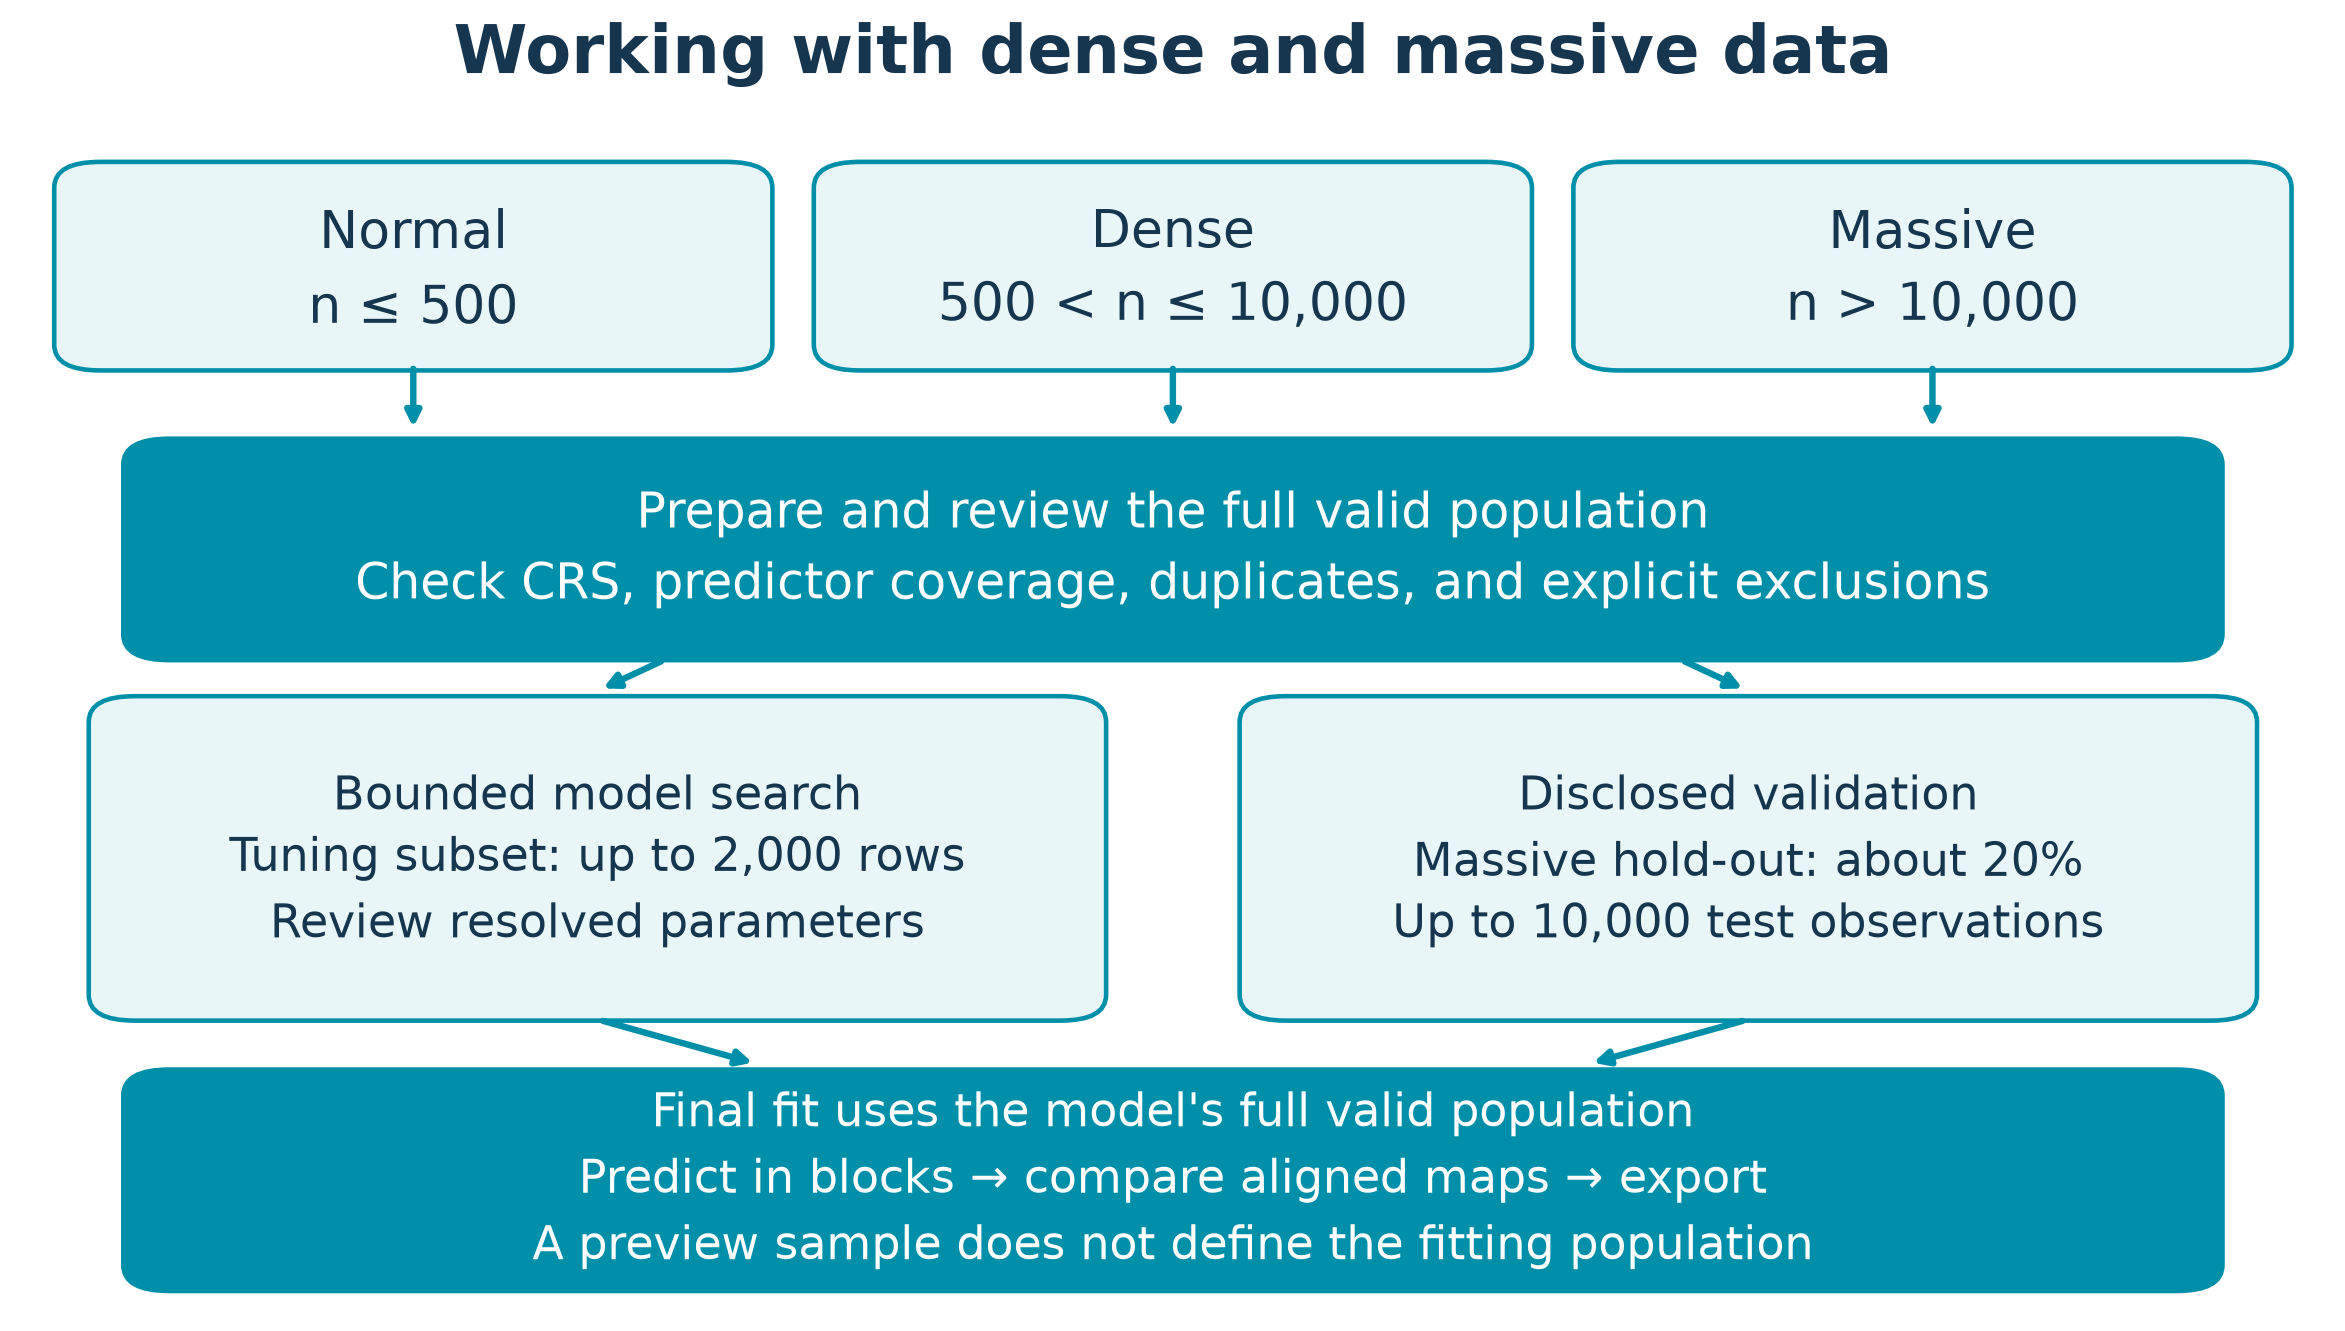
\includegraphics[width=0.97\textwidth,height=0.48\textheight,keepaspectratio]{dense_massive_workflow.png}
    \caption{Processing flow for dense and massive data: distinguish tuning, validation, final fitting, and display samples.}
    \label{fig:dense-massive-workflow}
\end{figure}

\subsection{Suggested Dense or Massive Workflow}

\begin{enumerate}
    \item Prepare the point values, projected CRS, boundary, and covariate coverage in QGIS. Remove duplicate coordinates before TPS and distinguish invalid measurements from legitimate extremes.
    \item Load the data and read the reported valid sample count and profile. Review suspicious observations through Outlier diagnostic and record any explicit exclusion decisions.
    \item Start with a practical pixel size. The number of grid cells scales approximately as mapped area divided by pixel area; halving the pixel width creates roughly four times as many cells.
    \item Prepare only the predictors needed for the objective. Missing predictor coverage reduces the training population and may leave NoData in the output.
    \item Evaluate candidate methods in Framework or fit one method manually. Review resolved tuning parameters, approximation notices, semivariogram settings, and the actual validation strategy.
    \item Run the final interpolation, then compare two validated maps on the same grid. Inspect local differences and the validation metrics before accepting the result.
    \item Review the interactive report and export the persistent raster and PDF needed for the project. Retain the source data, exclusions, parameter settings, profile, validation count, and software environment.
\end{enumerate}

\begin{infobox}
The massive profile makes large computations more manageable; it does not guarantee a runtime or make fine pixels statistically more informative. A denser map is still limited by the observations and predictors supporting it. Independent or appropriately spatial validation may be needed when the aim is transfer to unsampled areas.
\end{infobox}

\section{Practical Checks and Troubleshooting}

\begin{longtable}{P{0.30\textwidth}P{0.62\textwidth}}
\caption{Common situations and checks.}\label{tab:troubleshooting}\\
\toprule
\textbf{Situation} & \textbf{Action} \\
\midrule
\endfirsthead
\toprule
\textbf{Situation} & \textbf{Action} \\
\midrule
\endhead
Missing or blank inputs & Load the correct layers in QGIS, choose a numeric target, and click Load. A new plugin session starts from clean inputs. \\
Map or distance mismatch & Check metric CRS, polygon validity, sample overlap, pixel size, and covariate alignment before interpolation. \\
Suspicious observation & Inspect the original measurement and its neighborhood; a statistical or spatial flag alone does not exclude it. \\
No experimental points in REML & Expected behavior: REML displays the fitted theoretical curve only. Use MoM when experimental semivariances are needed. \\
Changed variogram settings & Recalculate or update the preview, rerun model validation, and apply a model evaluated under the current settings. \\
Unavailable comparison & Validate both candidate methods and resolve missing covariates or failed predictions. Comparison requires two aligned rasters. \\
Report shows an earlier method & The report describes the successful executed interpolation. Changing the next-run selection requires Run interpolation before the executed method changes. \\
Dense run takes too long & Inspect grid-cell count, predictors, neighborhood, and requested validation; begin with a coarser grid and the automatic profile. \\
Missing ML dependency & Use the plugin's compatible dependency setup for the current QGIS Python and architecture. Do not copy compiled packages from another 32-bit or 64-bit installation. \\
Need to retain the session & Export the raster and report and record exclusions and settings before closing; reopening intentionally starts a clean session. \\
\bottomrule
\end{longtable}

\clearpage
\begin{thebibliography}{99}
\raggedright


\bibitem[ANSELIN(1995)]{anselin1995}
ANSELIN, L. Local Indicators of Spatial Association: LISA. \textbf{Geographical Analysis}, v. 27, n. 2, p. 93--115, 1995. DOI: \url{https://doi.org/10.1111/j.1538-4632.1995.tb00338.x}.

\bibitem[BIER; SOUZA(2017)]{bierdesouza2017}
BIER, V. A.; SOUZA, E. G. de. Interpolation selection index for delineation of thematic maps. \textbf{Computers and Electronics in Agriculture}, v. 136, p. 202--209, 2017. DOI: \url{https://doi.org/10.1016/j.compag.2017.03.008}.


\bibitem[DELGADO BEJARANO et al.(2026)]{delgadobejarano2026}
DELGADO BEJARANO, L.; OLIVEIRA, A. L. G.; POZZUTO, J. V. F.; SÁNCHEZ, D. C.; AMARAL, L. R. do. Performance of interpolation methods in digital soil mapping: the influence of data characteristics. \textbf{Precision Agriculture}, v. 27, n. 1, article 10, 2026. DOI: \url{https://doi.org/10.1007/s11119-025-10311-8}.


\bibitem[KERRY; OLIVER(2007)]{kerryoliver2007}
KERRY, R.; OLIVER, M. A. Comparing sampling needs for variograms of soil properties computed by the method of moments and residual maximum likelihood. \textbf{Geoderma}, v. 140, n. 4, p. 383--396, 2007. DOI: \url{https://doi.org/10.1016/j.geoderma.2007.04.019}.


\end{thebibliography}
\end{document}
